\documentclass[
  final,
  pagePreset=largepage,
  babelLanguage=british,
  %webversion,
]{anecdote}

%\usepackage{local}

%% Details of the book
%% ===================

\title{Escuta Interior}
\subtitle{meditação no som do silêncio}
\author{Ajahn Amaro}
\publisher{The Publisher}
\date{2016-05-31}
\editionInfo{}
\ISBN{000-0-000000-00-0}

%% === Load further packages ===

%% === Hyphenation exceptions and corrections ===

% \hyphenation{}

\begin{document}

\frontmatter

\ifwebversion
\webcover{%
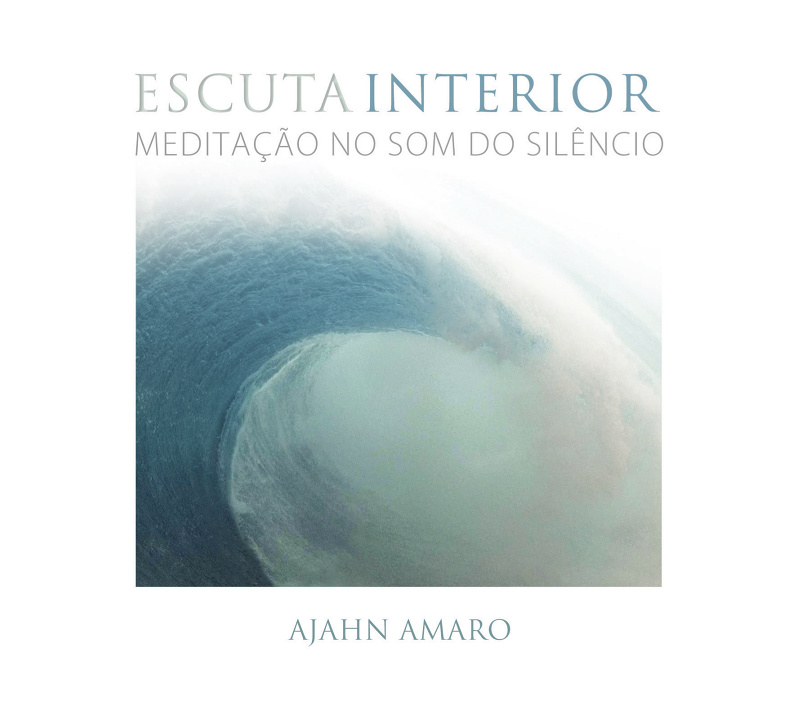
\includegraphics[height=\paperheight]{./webcover.jpg}%
}
\fi

\cleartorecto
\thispagestyle{empty}
\vspace*{2em}

{\centering

\resizebox{85mm}{!}{\Large\crimsonFont
\textls*{\color{gray!50}ESCUTA\space\color{gray!80}INTERIOR}}

\vspace*{8pt}

\resizebox{85mm}{!}{\firaSansLightFont
\color{gray!40}%
\textls*{\MakeUppercase{meditação no som do silêncio}}}

\vfill

{\large\crimsonFont\color{gray!80}%
\textls*{AJAHN AMARO}}

\vfill

\mbox{}

}


\cleartoverso
\thispagestyle{empty}

\enlargethispage{3\baselineskip}

\vspace*{-3\baselineskip}

{\copyrightsize
\centering
\setlength{\parindent}{0pt}%
\setlength{\parskip}{0.8\baselineskip}%

\thetitle\\
por \theauthor

Publicações Sumedhārāma\\
\href{http://sumedharama.pt}{www.sumedharama.pt}

Para distribuição gratuita\\
\textit{Sabbadānaṃ dhammadānaṃ jinati}\\
‘A oferta de Dhamma é superior a qualquer outra oferta.’

Este livro encontra-se disponível para distribuição gratuita em\\
\href{http://fsbooks.org/}{www.fsbooks.org}

ISBN \theISBN

Copyright \copyright\ Publicações Sumedhārāma 2017

Tradução: Helena Gallis\\
Editor: Appamādo Bhikkhu\\
Formatação: Gambhīro Bhikkhu

\vfill

Publicado originalmente em 2012 pelas Publicações de Amaravati\\
Copyright \copyright\ Amaravati Publications 2012\\
Para permissão para reimprimir ou traduzir é favor contactar\\
Amaravati Publications em publications@amaravati.org\\
Se desejar traduzir este texto deverá fazê-lo a partir do texto original em Inlglês.

Este trabalho está licenciado com uma Licença Creative Commons\\
Atribuição-NãoComercial-SemDerivações 4.0 Internacional.

Veja página \pageref{copyright-details} para mais detalhes sobre direitos e restrições desta licença.\\
Produzido com o sistema tipográfico \LaTeX. Fonte utilizada: Gentium, Fira~Sans e Crimson~Roman.

\theEditionInfo

}


\cleartorecto
\tableofcontents*

\mainmatter

% Escuta Interior
\chapter{Escuta Interior}

Há um certo número de temas que são familiares a quem pratica a
meditação budista: `consciência da respiração', focando-se no ritmo da
respiração; `meditação a andar' que gira à volta dos passos que se dá
para cima e para baixo; a repetição interna de um mantra, como por
exemplo, `Bud-dho' -- todos eles servem para fixar a atenção na presença
do próprio momento, na realidade presente.

A par destes métodos mais conhecidos existem muitos outros com uma
função semelhante. Um deles é conhecido como `escuta interior' ou
`meditação no som do silêncio', ou em sânscrito: \emph{nada yoga}. Toda
esta terminologia refere-se a estar atento ao que se chamou o 'som do
silêncio', ou o `som \emph{nada}'.

\emph{Nada} é a palavra sânscrita que significa `som', mas também a palavra
espanhola e portuguesa para `a ausência de algo' -- uma interessante e acidental
coincidência plena de significado.

% TODO review: a palavra espanhola e portuguesa -- note not necessary
% *N.T.(nota da tradutora)

\section{O Som Interior e Como Encontrá-lo}

O som \emph{nada} é um tom interior de vibração de elevada frequência.
Se dirigirem a atenção para a audição, se ouvirem com muito cuidado os
sons à sua volta, escutarão um som contínuo de alta frequência, como que
um som branco -- sem começo, sem fim -- cintilando bem dentro, lá no
fundo.

Vejam se conseguem discernir esse som e focar-se nele. De momento não é
preciso teorizar sobre ele ou divagar sobre o que será exactamente,
decidam apenas centrar-se nele. Tentem detectar essa tão delicada
vibração.

Se forem capazes de ouvir esse som interior, poderão usá-lo tão
simplesmente como qualquer uma outra forma de meditação. Pode ser usado
tal como a respiração como um objecto de consciencialização. Centrem
nele a atenção e permitam que preencha toda a esfera da vossa
consciência.

\section{As Duas Dimensões de Samādhi}

A concentração meditativa, \emph{samādhi}, pode ser descrita como `um
objecto mental capaz de preencher a consciência durante um certo tempo',
ou `fixar a mente num só objecto'. Por consequência, \emph{samādhi} é
uma forma de se focar num único objecto, mas que, sendo ímpar, pode
funcionar de duas maneiras. Primeiro, podemos vê-la como `o ponto que
exclui', ou seja, reduz-se a um só objecto e põe de fora tudo o resto à
sua volta. Assim, esta forma é de uma fixação firme e estreita,
semelhante ao foco concentrado de uma lanterna ajustável. Esta é a base
de \emph{samatha}, o que significa calma ou tranquilidade.

A segunda forma pode ser chamada de `o ponto que inclui', ou seja,
trata-se de uma consciência expansiva que faz da totalidade do momento
presente o objecto de meditação. Permite-se que o `ponto único' se
expanda até englobar todos os padrões da experiência presente, tal como,
quando usamos o foco alargado da mesma lanterna ajustável todos os
objectos nesse momento são abrangidos pela luz da consciência, mais do
que existir, apenas, um foco de luz brilhante. Esta é a base do
\emph{vipassanā}, ou da realização.

Uma das grandes bênçãos da meditação do som interior é a capacidade de
suster facilmente estes dois tipos de \emph{samādhi}: tanto o ponto que
exclui, como o ponto que inclui.

\section{Nada Como Sustentáculo da Tranquilidade -- Samatha}

Podemos fazer do som interior um objecto fundamental de atenção,
permitindo que preencha todo o espaço do conhecido. Com plena
consciência, largamos tudo o mais -- as sensações no corpo, os ruídos
que ouvimos, os pensamentos que surgem -- colocando-os na periferia, nas
orlas do nosso foco de interesse. Em sua substituição, permitimos que o
som interior preencha completamente o foco da nossa atenção, o espaço
desta consciência, sustentando directamente a consolidação de
\emph{samatha}, a tranquilidade. Podemos usá-lo tal como fazemos com a
respiração, para dominar a atenção, e ser um objecto único que ajuda a
centrar, estabilizar, a dar firmeza - uma unidade de atenção no
presente.

\section{Nada Como Um Sustentáculo da Realização -- Vipassanā}

Se nos focarmos no som interior durante tempo suficiente até se tornar
firme e constante, mantendo com facilidade a mente no presente,
permitiremos então que o som se desloque lá para o fundo. Desta forma o
som é como um ecrã, onde todos os outros sons, sensações físicas,
estados de espírito e ideias são projectados -- tal como uma tela onde é
exibido o filme dos restantes padrões da nossa experiência. E por ser
plano, uniforme, é um bom ecrã. Não interfere, nem se confunde com
outros objectos que vão surgindo, e, contudo, é tão obviamente presente.
É como se fosse uma tela ligeiramente salpicada, ou uma tela especial,
na qual é projectado um filme, e por conseguinte, se estiver atento,
notará que existe um écran onde a luz é projectada. E tal vem
lembrar-lhe que só se trata de um filme - é só uma projecção, não é
real.

Podemos simplesmente deixar que o som permaneça nos bastidores, e essa
presença, por si só, é um lembrete. Sustenta a memória, ``Ah pois é: são
apenas \emph{sankhāras}, formações mentais, que chegam e partem. Todas
as formações são insatisfatórias -- \emph{sabbe sankhārā dukkhā.} Se
alguma coisa se forma, se é `algo', existe uma qualidade de
\emph{dukkha} na sua impermanência, na sua própria existência como
`algo'. Por isso não se apeguem, não se enredem, não se identifiquem,
não o vejam como vosso, ou quem são, ou o que são. Larguem.''

A presença do som pode, por conseguinte, facilitar a forma como cada
\emph{sankhāra --} seja uma sensação física, um objecto visual, um
humor, um estado refinado de felicidade, ou o que for, - seja vista como
vazio e sem dono. Tal ajuda a sustentar uma objectividade, uma
consciência liberta, uma forma de participação imparcial no presente.

Dá-se o fluir do sentir, o peso do corpo, a sensação das roupas, o fluxo
dos humores, o cansaço, a dúvida, a compreensão, a inspiração, o que
seja, mas o \emph{nada} ajuda a suster a objectividade clara por entre
os padrões de humores, de sensações e de pensamentos.

Permite que o coração repouse numa condição de consciência plena, sendo
essa mesma consciência conhecedora que recebe a corrente da experiência
-- a que sabe disto, a que se liberta dela, a que reconhece a sua
transparência, o seu vazio, a sua falta de substância.

O som interior prossegue nos bastidores, lembrando-nos que tudo é
\emph{Dhamma}, tudo é um atributo da natureza, que vem e vai, que muda,
e nada mais que isso. Esta é a verdade, que, quiçá, tenhamos intuído há
muito tempo, mas que entretanto esquecemos por nos enredarmos com a
nossa personalidade, as nossas memórias, estados de espírito e
pensamentos, desconforto do corpo e apetites.

A tensão criada pelo apego às experiências diárias desde o nascimento,
vai confundindo, iludindo e enfeitiçando a atenção. Não obstante,
podemos usar a presença do som \emph{Nada} para ajudar a quebrar a
ilusão, e terminar com o encantamento, e ajudar-nos a reconhecer a
corrente das sensações e dos humores pelo que são: padrões da natureza,
chegando e partindo, mudando, actuando à sua maneira. Não são quem, ou o
que, nós somos, e nunca nos poderão satisfazer, nem desapontar, se os
virmos intuitivamente.

\section{Nada Permite Escutar Os Pensamentos}

Consoante vai desenvolvendo a escuta interior, usando a meditação
formal, começa a notar como o facto de escutar um objecto audível ajuda
a escutar de forma objectiva os pensamentos, os estados de espírito.

De certa forma, o tagarelar do pensamento não tem mais significado que o
sibilar cintilante do som \emph{nada}. São tão-somente as vibrações da
mente pensante dando forma a padrões conceptuais, só isso -- apenas uma
murmurante corrente de vibrações prolongada e contínua. Podemos, assim,
aprender a ouvir o nosso pensamento, tal como escutaríamos uma corrente
de água, uma queda de água, ou uma música coral de um bando de aves, com
o mesmo tipo de ausência de envolvimento ou de identificação. Não é mais
que um ribeiro murmurante na mente. Nada de mais - não suscita nada, nem
perturba.

Tudo isto é muito fácil de dizer, mas efectivamente temos a tendência
para nos envolver nas nossas histórias, não é? Adoramos histórias,
particularmente histórias sobre nós: o bem e o mal que fizemos, o
memorável, o doloroso, o lamentável, o que queremos fazer, o que
esperamos, o que receamos, o que os outros pensam de nós\ldots{}

Estes prezados padrões são todos manifestações do elemento 'eu', hábitos
de pensamento de toda uma vida, em termos de `eu', `mim 'e `meu'. Em
Pali são chamados de \emph{ahamkāra}, `criador de eu' e
\emph{mamankāra}, 'criador de meu', sendo eles as características-chave
da visão pessoal. Estes hábitos são o que mais repetida e efectivamente
dirige a nossa atenção para o domínio conceptual, levando, por sua vez,
à dispersão da mente. Se a história tiver um eu, torna-se muito mais
interessante que qualquer outra história remota. Tudo isto é
extremamente natural, um hábito básico de todos nós.

Por conseguinte, grande parte da meditação intuitiva, o desenvolvimento
de \emph{vipassanā,} só trata disso - aprender a reconhecer os hábitos
dos `criadores do eu e do meu' nos pensamentos que temos.
\emph{Ahamkāra} significa literalmente `feito de si próprio', enquanto
\emph{mamankāra} significa `feito de mim próprio'; a verdadeira intuição
é o reconhecimento desses hábitos, não se deixar levar pela história --
saber ver neles o vazio e a transparência, e libertar-se deles.

\section{Nada, Vazio e Verdade}

A maioria dos praticantes do Budismo, independentemente da tradição,
estão familiarizados como que se chama `as três características da
existência' -- \emph{anicca, dukkha, anattā} (impermanência,
insatisfação e não-eu). Estas são as qualidades universais de todas as
experiências que surgem e desaparecem, e admitir a sua presença é o
aspecto mais vivo da meditação \emph{vipassanā.}

Existem, contudo, outras características universais da existência que, à
semelhança, podem ser usadas para ajudar o coração a libertar-se de toda
a limitação, peso e tensão. Duas destas características, operando como
num par, são chamadas de \emph{suññatā} e \emph{tathatā}, significando
respectivamente, vazio e Verdade. O termo `vazio' deriva de dizer `não'
ao fenómeno do mundo: «Não vou acreditar nisto -- é oco, vazio, não tem
nada, não é propriamente real.»

A `Verdade' é uma qualidade que corresponde a `vazio', da mesma forma
que a direita combina com a esquerda. Contrastando, porém, com a sua
parceira a sua natureza deriva de dizer `sim' ao universo. Poderá não
haver aqui nada de sólido, separado ou individual -- quer seja um
pensamento, um narciso ou uma montanha -- existe, contudo, algo, há aqui
uma Realidade Última que sustenta, permeia, abrange e constitui tudo. A
palavra `Verdade' expressa, assim, um apreço à natureza dessa Realidade,
e a sua tomada de consciência pode ser caracterizada pelo conhecimento e
materialização da presença do Incondicionado, o Imortal, ou
\emph{amata-dhamma}.

Quando se fala de vazio no \emph{Canon Pali,} as escrituras do mundo do
Budismo do sul, geralmente significa `o vazio do eu e do que pertence ao
eu', mas também se refere à insubstancialidade dos objectos. Quando se
desenvolve a capacidade da escuta interior e de seguir o som
\emph{nada}, potencia-se a compreensão quer do sujeito, quer do objecto,
quer do `eu', quer do `outro'.

Quando se firma na escuta do som \emph{nada} de uma forma estável, sendo
o seu tom cintilante de prata já uma presença constante, percebe-se quão
fácil é o reconhecimento da ausência de substância de todo o `eu',
`mim', ou 'meu', origem das atitudes e dos pensamentos, como já descrito
anteriormente. É como que uma luz brilhante, através da qual conseguimos
ver com clareza o oco nas bolhas de ar que flutuam.

De forma análoga, para todos os objectos mentais que são vividos -- tais
como o que vemos, ouvimos, cheiramos, saboreamos e tocamos, bem como as
memórias, planos, humores e ideias que surgem na mente -- a presença do
som \emph{nada} ajuda a iluminar a transparência de todos estes padrões
de consciência. O Buda disse-o desta forma:

\begin{quote}
A forma material é como espuma\\
Tocando uma bolha de água;\\
A percepção é só uma miragem,\\
Volições semelhantes a um tronco de planta,\\
Consciência, um truque de magia --\\
Assim diz o Parente do Sol.\\
Contudo, deve-se ponderar\\
Ou indagar cuidadosamente,\\
Afinal tudo é vazio e vago\\
Quando visto verdadeiramente

\emph{S 22.95}
\end{quote}

O som \emph{nada} também pode ajudar a relembrar a Verdade de todas as
experiências. Embora estes predicados possam parecer contraditórios,
será mais correcto dizer que são complementares. Quando se escuta
atentamente o som do silêncio e se permite que preencha o espaço
interior da consciência, a sua qualidade energética juntamente com a
riqueza informe de sua presença, é uma forte lembrança intuitiva da
condição da Verdade. É como se (pelo menos para quem fala inglês) o som
interior se expressasse num `\emph{iiiissssss}'\ldots{}, ou
\emph{`thussss\ldots{}}' infinito, que o traz de novo à realidade.

A Verdade é, por definição, conceptualmente difícil de explicar, possui
uma característica intrinsecamente incompreensível que pode parecer vaga
ou irreal, mas que, ironicamente, se torna parte necessária do seu
significado. É bem significativo o facto de Buda ter atribuído a si
próprio a expressão \emph{Tathāgata} -- que significa tanto `O que
alcançou a `Verdade' como `O que foi para a Verdade', dependendo da
interpretação. Assim, mesmo que a palavra `Verdade' possa trazer um tom
intangível (ao som do silêncio), tal é deliberado, e deve ser
reconhecida como expressão de uma realidade fundamental.

Pode-se fazer uma comparação com o mundo da matemática, usando o
conceito da raiz quadrada de -1. No mundo dos números reais não há
nenhum número inteiro que se possa multiplicar por si próprio para
produzir -1. Se, contudo, tal número existisse, todo o tipo de
possibilidades interessantes se abririam, como foi descoberto há muito
tempo, e desenvolvido pelos matemáticos do séc.XVIII.

É intrigante, mesmo sabendo que este número não existe no mundo real, só
tendo um estatuto imaginário, como se torna essencial na construção dos
deslocamentos de fase (atraso de propagação) dos osciladores, usado na
engenharia do som, estendendo-se o seu uso aos gráficos informatizados,
à robótica, ao processamento de sinal, simulações informatizadas e à
mecânica orbital.

Em conclusão, tal como acontece com a essência, mesmo que seja
indescritível, tem uma presença clara e demonstrável no mundo real.\cite{imaginary}

\section{Nada e `Atammayatā' -- Ver o Mundo Na Mente}

A terceira característica da existência, uma característica ainda mais
subtil, é chamada de \emph{`atammayatā'}. Significa literalmente `não
feito disso'.

Quando se consideram as características do vazio e da essência, ainda
que o conceito do `eu sou' -- \emph{asmi-manā} -- possa já ter sido
esclarecido, ainda podem restar alguns traços subtis de apego;
agarrarmo-nos à ideia de um mundo objectivo ser reconhecido através de
um mundo subjectivo, mesmo sabendo que não existe nenhum sentido de `eu'
discernível. Pode restar a sensação de um `isto' que conhece um `isso',
tal como dizer `sim', no caso de Realidade Intrínseca, e `não' no caso
de vazio.

\emph{Atammayatā} é o desfecho de todo esse domínio. Exprime a
realização de que, `não existe \emph{Isso}'. É o colapso genuíno tanto
da ilusão da separação entre o sujeito e o objecto, como da
discriminação entre os fenómenos, vistos como substancialmente
diferentes entre si.

Uma forma que permite desenvolver esta realização a um nível prático é a
de combinar a escuta do som \emph{nada} com a seguinte simples reflexão:

A nossa tendência é de olhar para a mente como algo que existe no corpo.
Na verdade, entendemos mal: o corpo é que existe na mente. Tudo o que
conhecemos do corpo, de agora e de antes, foi conhecido pela actividade
mental. Com isto não se pretende dizer que não existe um mundo físico,
mas o que temos como seguro, é que a experiência do corpo e a
experiência do mundo provêm da mente.

Tudo acontece aqui. E quando `o aqui' é verdadeiramente reconhecido e
despertado, a noção do mundo como algo externo, a noção de separação,
cessa. Quando nos apercebemos que o mundo está dentro de nós, a noção de
o mundo ser algo apartado de nós desvanece-se permitindo-nos uma melhor
compreensão da sua verdadeira natureza.

Se se focar no som interior e depois simplesmente reflectir, lembre-se
que `O mundo está na minha mente. O meu corpo e o mundo existem neste
espaço de consciência, permeados pelo som do silêncio', o que poderá
proporcionar-lhe uma mudança de visão. Com este domínio, acaba por ver o
seu corpo, a mente e o mundo todos numa só resolução: a compreensão da
ordenada perfeição. O mundo está equilibrado dentro desse coração pleno
de vibrante silêncio.

\emph{Atammayatā} é a premissa interna que sabe que `Não existe qualquer
``\emph{isso}''. Só existe ``\emph{isto}''.' E, quando se realiza esta
verdade, até a condição de `isto', e de `aqui' passa a não ter
significado. A presença do som \emph{nada} ajuda a realizar e a manter
tal perspectiva. Desta forma, pouco a pouco, a mente vai perdendo o
hábito de querer exteriorizar-se, de ser apanhada nas suas tendências
nefastas, \emph{āsava}, e, assim perder-se nas preocupações do mundo.
Desenvolve-se uma confortável contenção, uma compostura interna e uma
ausência de compulsões que, com tanta facilidade, perturbam o coração
confundindo e bloqueando-nos.

\emph{Atammayatā} ajuda o coração a libertar-se dos mais subtis hábitos
de inquietação e serena as reverberações das ilusões enraizadas na
dualidade sujeito-objecto. Essa tranquilidade traz ao coração a
compreensão de que só existe a integralidade do Dhamma, a noção de
espaço pleno e de realização. As aparentes dualidades disto e daquilo,
sujeito e objecto, passam a não ter qualquer significado.

\section{Nada Abrange Actividade e Compromisso}

Quando já tiver desenvolvido uma atenção estável ao som \emph{nada} na
posição formal sentada, poderá alargá-la para também fazer parte da
meditação a andar. Notará que, embora de olhos abertos e com o corpo a
caminhar firmemente para a frente e para trás entre os dois limites do
trilho definido para a meditação a andar, consegue ouvir o som
\emph{nada} abrangendo tudo. Lá está ele, solidamente lá no fundo,
permeando toda a experiência e relembrando-o que tudo isto se torna
entendível dentro da esfera da sua consciência. O corpo e o mundo estão
indubitavelmente dentro da mente.

Ao tornar-se um adepto na manutenção da atenção usando o som do silêncio
nestes variados objectos, entenderá que poderá usá-lo em quase todas as
situações. A sua atenção torna-se mais robusta.

Se estiver a caminhar na rua, a brincar com os filhos, à espera de uma
reunião de negócios, a comer uma refeição, em pé numa fila, a falar com
amigos, a ver TV, a escrever um artigo, ao visitar a sua mãe\ldots{} até
mesmo no meio de uma actividade ruidosa ou na presença de barulhos
estridentes, como trânsito intenso, a proximidade de uma serra eléctrica
ou de um martelo pneumático, se escutar, lá está ele. Podemos, assim,
usá-lo sempre como um suporte para a plena atenção e perfeita
consciência.

Além disso, se for usado como um lembrete para obter perspectivas mais
adequadas, ajuda a relacionar-se com a actividade em questão, de uma
forma mais sensível. Parece que amplia a atenção, mais do que dividi-la.
Acrescido a isto, ao prestar-lhe atenção no meio das actividades e dos
compromissos, permite-lhe viver as situações sem a obstrução das
preocupações egóicas.

Está a conceder a si próprio uma oportunidade de responder
conscientemente aos inumeráveis acontecimentos e experiências da vida,
de acordo com as leis da natureza, mais do que a reagir cegamente, por
via dos hábitos e das compulsões. Pode libertar-se dos infindáveis
ciclos de impulsos e de arrependimentos, nos quais a maioria de nós se
sente enredado.

\section{Nada e o Desenvolvimento Da Compaixão}

Além de ajudar o coração na libertação de tendências tão obstrutivas, e
de defender qualidades tão saudáveis no meio de actividades e
compromissos, a presença do som \emph{nada} também pode ser usada para
estimular e manter a bondade e a compaixão. Se considerarmos o quanto
recebemos e nos empenhamos com o mundo em geral, estes são os predicados
mais abençoados e proveitosos que devemos cultivar.

É de realçar que o Bodhisattava Guan Yin, Avalokiteshvara, na tradição
do Budismo do Norte, corresponde ao papel da encarnação da compaixão. O
seu nome significa `Aquele que Escuta os Sons do Mundo', e tendo em
conta isto, dá-nos uma notável indicação sobre a origem das raízes da
compaixão. Ainda que possamos registar o conceito de compaixão como
sendo prioritariamente `actuar no sentido de ajudar os seres que
sofrem', este nome (e, sem dúvida, a prática de meditação recomendada
por Guan Yin, como descrita abaixo) aponta para o predicado central,
como sendo mais de receptividade e de harmonização com o estado das
coisas. Assim, através de tamanha e atenciosa aceitação, as mil mãos de
Guan Yin podem dar início ao trabalho.

As características do Bodhisattva são um símbolo espiritual orientador
de caminhos possíveis de trabalhar. Podemos assumir a prática de ouvir o
som interior e usá-lo como forma de ajudar a expressar compaixão na
vida. Abrindo o coração ao som do silêncio e libertando-nos de outras
preocupações, conseguimos estar em plena consciência e sabiamente
atentos ao momento presente e a tudo o que ele contém; usando essa plena
consciência, a disposição inata de compaixão, no coração puro, desperta:
e então, essa atitude compassiva toca os seres que nos rodeiam.
Acrescido a isto, o simples treino de escutar tem o seu próprio impacto
na forma como nos relacionamos com os outros. Foi já explicado como o
ouvir o som do silêncio ajuda na observação dos pensamentos; ora bem,
tal acaba por ser igualmente eficaz na capacidade de escutar os outros.
A bondade e a compaixão requerem muita paciência e aceitação, e a
prática de saber escutar é um meio poderoso para as fazer germinar e
moldar. Tentar ouvir os outros -- sem reagir, sem se envolver, sem se
desligar, sem se enfadar -- é uma arte e uma graça. Acompanhar o que o
outro está a dizer e, nisto, recebê-lo completamente, é uma bênção para
ele e para si.

Numa visão alargada, podemos estender esta atitude de atenção
compassiva, e passar a escutar os sons do mundo, de tal forma que o
coração aprenda a abraçar todos os seres e suas labutas. Note-se que não
se trata de um abraço hipotético, mas antes -- tal como o
Avalokiteshvara não só ouve, mas possui muitas cabeças, mãos, olhos e
competências -- de harmonizar os nossos corações com o mundo inteiro
originando actos e palavras que auxiliem sob formas mais práticas e
tangíveis. Ao aprender a escutar o som do silêncio desta maneira -- sem
paixão, aversão ou enfado -- estamos a incrementar uma via directa para
a bondade e a compaixão, atitudes que concedem um sublime espaço eterno
ao coração, e que iluminam o mundo com tanta beleza.

\section{Nada Ajuda a Ver Pela Visão Pessoal}

Uma das obstruções principais a tão ilimitadas atitudes, é a fiel
perturbadora, visão pessoal. Felizmente podemos usar o som interior, o
\emph{nada}, para reforçar a visão desse hábito mental criador de
pessoalidade, bem como a obsessão para o regenerar continuamente.

Uma prática que pode ajudar o coração a libertar-se de tal impulso, é
meditar no seu próprio nome. Comece por escutar o som interior por um
momento. Concentre-se nisso até a mente aclarar e se abrir, vazia, e
então pronuncie simplesmente o seu nome, internamente, qualquer que seja
o nome. Antes escutara o som do silêncio, depois o som do silêncio
dentro, e depois por detrás, do seu nome, e por fim o som do silêncio
após o ter repetido. 'A-ma-ro', `Su-san', `John'. Veja o que é que esse
som lhe traz. É só o som do seu nome, tão familiar, tão vulgar; para
variar, veja o que acontece quando ele se deixa cair no silêncio da
mente e é realmente sentido e percebido. Veja o que é que faz, se
descortina o hábito de se ver sob alguma forma em particular, abrindo
fronteiras. Para nossa surpresa, esse nome, essas sílabas tão
familiares, subitamente pode sentir-se como a mais peculiar, a mais
estranha formulação do mundo. Algo se agita e intui no coração, «Afinal
que relação é que isso tem com algo real?». Nesse momento compreendemos
que a palavra que forma o nosso nome e que é normalmente usado para nos
referir é, efectivamente, uma condição completamente impessoal.
Proferir, desta maneira, o nosso nome, no inequívoco espaço aberto da
sabedoria, pode ser percebido como tentar escrevê-lo com um feixe de luz
numa catarata. Não existe nada com que registar, nem onde registar.

Este tipo de prática pode ser tão ligeiramente perturbador, quão
gloriosamente libertador, e se consentirmos que nos liberte, tudo o que
resta é esse sabor de liberdade, e o som da água a cair.

\section{Nada e o Questionar-se}

Outra forma, quiçá mais directa, que pode ser usada ao escutar é a de
questionar-se, com o sentido de abordar e dissolver hábitos de visão
pessoal.

Mais uma vez, escute o som do silêncio, foque-se nele para centrar a
atenção com firmeza, que a mente fique o mais silenciosa e alerta
possível, e depois coloque-se a questão: «Quem sou eu?»

Inicialmente ouça o som do silêncio, a seguir questione-se e depois
aguarde; repare no que acontece quando coloca com sinceridade essa
questão «Quem sou eu?». Não estamos, explicitamente, à espera de uma
resposta verbal, de uma resposta conceptual; repare, contudo, que existe
um hiato, um hiato breve entre o tempo que decorre depois de colocarmos
a questão e antes de surgir qualquer tipo de resposta verbal,
conceptual. Quando verdadeiramente colocamos essa pergunta «Quem sou
eu?», ou «O que é que sou?», há um hiato, um espaço que se abre por
breves momentos, onde o coração intui, se abre à dúvida sobre as
presunções que temos vindo a fazer sobre ser-se alguém: homem, mulher,
novo ou velho.

Dá-se um momento de espanto antes de todos os detalhes pessoais
começarem a desaguar. Há um intervalo, uma hesitação - «Quem sou eu?»

Deixe a sua atenção repousar nesse intervalo depois do fim da pergunta e
antes de surgir a resposta. Firme a atenção nesse intervalo, nessa
dimensão, e verá, em boa verdade, que o silêncio da mente é a resposta à
questão. Permita e incentive a mente a ficar nessa amplitude aberta,
atenta e desconstruída, pois nesse momento a visão pessoal é
interrompida. Os hábitos normais de criação do ego são confusos,
reprovadores. O hábito de criar o ``eu'' é apanhado no acto. De repente
a câmara volta-se para o fotógrafo, antes que possa escapar. É o momento
desconstruído, descondicionado. A atenção surge e a mente fica alerta,
pacífica e luminosa. Mas sem qualquer sentido de eu. É algo tão
extraordinariamente simples e natural. Fixe a atenção aí.

Passado algum tempo, quando começam a surgir outras preocupações -- uma
dor na perna, o som do carro a passar, uma cócega no nariz - quando as
visões pessoais começam a reajustar-se, regresse ao som \emph{nada},
escute e ponha de novo a pergunta: «Quem sou eu?», abrindo aquela janela
da curiosidade, da realidade, perfurando a bolha da visão do ``eu'', só
por um momento. Repare no que se passa, assim que a bolha já não ofusca
ou distorce a nossa visão das coisas, e a visão pessoal cai por terra -
O que fica? O que é a vida quando se interrompe esse hábito?

Tal como a meditação no nosso nome, esta prática pode ser
simultaneamente uma ameaça e um alívio. Todavia, se não nos deixarmos
distrair por qualquer um desses sentimentos, e permanecermos
simplesmente atentos e abertos ao presente, o que se realiza é a pureza,
a radiância, a paz, uma normalidade original e uma simplicidade
abençoada, tudo envolto no silêncio ululante.

\section{Os Atributos De Nada}

Vários atributos do som \emph{nada} manifestam qualidades espirituais
muito úteis, algumas das quais permitem que sejam, pelo menos,
universalmente acessíveis e profícuas no que se refere, quanto mais não
seja, à concentração na respiração.

Primeiro, ao usar o som \emph{nada} como um objecto de meditação,
estimula-se a atitude de escuta e receptividade. Exige que, mais do que
dirigir uma actividade, se vivencie de coração aberto.

Segundo, o som não está sujeito ao controlo pessoal. Diferente da
respiração, que podemos alongar, encurtar, ou mudar segundo a nossa
vontade, não podemos tornar o som interior mais estridente ou mais
suave, fazer com que acabe ou comece, ou qualquer outra coisa. Podemos
focar-nos nele ou não, mas não está sujeito a direcções ou escolhas
pessoais. Na verdade, incita-nos naturalmente à realização na mais
profunda impessoalidade -- sem qualquer característica particular que
nos leve a pensar em ``mim'' ou ``meu''. Não é feminino, nem masculino,
novo nem velho, inteligente nem estúpido\ldots{}não tem tamanho nem
nacionalidade, nem cor nem língua\ldots{} existe, tão simplesmente, na
imparcialidade da Natureza.

Por fim, é energizante, possui uma qualidade que estimula naturalmente.
Quanto mais atenções lhe dermos, mais lúcida se torna a mente. Funciona
como um circuito de feedback positivo, de tal forma que, quanto maior
atenção se lhe der, mais reforçada será a capacidade de ficar atento.
Suporta, assim, o próprio acto de meditar, ao ajudar a mente a ficar
mais alerta.

\section{Nada Como Um Símbolo De Transcendência}

O som do silêncio é um objecto do domínio sensorial que reflecte muitas
características do Dhamma, como condição transcendente, e por
consequência, pode actuar como uma presença simbólica para tal, e ser
uma forma de recordar essa Verdade Última.

Por exemplo, o som \emph{nada} está sempre ``aqui''. Desta maneira, é um
bom símbolo para condição \emph{sanditthiko} do Dhamma, i.e., imanente,
presente aqui e agora''. De igual modo, não tem princípio nem fim, o que
representa muito bem a qualidade do Dhamma -- \emph{akāliko --} a
intemporalidade. É impessoal, sempre presente.

Assim que repararmos nele, instiga à investigação, ressoando, assim, o
atributo do Dhamma \emph{ehipassiko}, ``o que convida a vir ver''.

Conduz à interiorização, desmotivando o interesse de se deixar absorver
pelo mundo dos sentidos, daí a qualidade \emph{opanayiko} do Dhamma ser
igualmente bem representada.

Por fim, dá iniciativa àqueles que se interessam por presenciar e
valorizar tudo isto, daí \emph{paccattam veditabbo viññūhī --} ``a ser
conhecido por cada sábio, por si próprio'' -- é perfeitamente adequado a
esse atributo.

Consequentemente, ainda que seja um simples objecto sensorial, pelo
menos dentro do sistema filosófico do Budismo, os seus atributos
conferem um delicado símbolo ao Dhamma em si -- uma ressonância, se
quiser, no reino dos sentidos das qualidades fundamentais e
transcendentais da Verdade Última.

\section{Nada e Suas Diferentes Manifestações}

Posto tal, é um facto que há quem tenha muita dificuldade em discernir
este som interior. Por isso, ao ler isto, poderá estar a cogitar, «Mas
afinal de que é que ele está a falar?»

Nem toda a gente consegue captar com facilidade esta experiência no
domínio da audição. Tal acontece pelos nossos traços de carácter, onde
nos deixámos condicionar de outras formas, por exemplo se for um artista
plástico, essa vibração interior pode ser mais discernível em termos de
qualidade visual, uma oscilação subtil no campo visual. Ou, caso tenha
desenvolvido uma grande consciência corporal, como um professor de hatha
yoga, poderá sentir no corpo uma delicada e penetrante condição
vibratória, um retinir, um formigar nas mãos de uma presença de energia
subtil, uma corrente contínua vital pelo corpo.

A frequência com que o captamos depende dos condicionamentos, dos
hábitos e formações provenientes de cada \emph{karma} pessoal. Da minha
experiência pessoal do ensino deste método ao longo de vinte anos, a
maioria das pessoas discerne com mais facilidade no domínio da audição.
É por isso que se chama ``\emph{nada yoga'' --} o \emph{yoga,} ou
disciplina espiritual, do som -- contudo, se tiver mais facilidade em
captar essa vibração universal pela visão, ou pelo corpo, ou até mesmo
pelo paladar ou olfacto, é uma prática com igual viabilidade. Focar-se
na sua presença e nas dinâmicas de seus efeitos, funciona exactamente da
mesma maneira, independentemente do meio sensorial através do qual se
vivencia. Pode ser usado para todas as práticas acima descritas, e ainda
assim irá obter resultados equivalentes. Se essa for a sua disposição, é
aí que vai encontrar os resultados melhores, já diz o ditado: ``O ouro
vai estar onde o encontrar''.


% O Som Interior e Como Encontrá-lo
\chapter{O Som Interior e Como Encontrá-lo}

O som \emph{nada} é um tom interior de vibração de elevada frequência.
Se dirigirem a atenção para a audição, se ouvirem com muito cuidado os
sons à sua volta, escutarão um som contínuo de alta frequência, como que
um som branco -- sem começo, sem fim -- cintilando bem dentro, lá no
fundo.

Vejam se conseguem discernir esse som e focar-se nele. De momento não é
preciso teorizar sobre ele ou divagar sobre o que será exactamente,
decidam apenas centrar-se nele. Tentem detectar essa tão delicada
vibração.

Se forem capazes de ouvir esse som interior, poderão usá-lo tão
simplesmente como qualquer uma outra forma de meditação. Pode ser usado
tal como a respiração como um objecto de consciencialização. Centrem
nele a atenção e permitam que preencha toda a esfera da vossa
consciência.


% As Duas Dimensões de \emph{Samādhi
\chapter{As Duas Dimensões de \emph{Samādhi}}

A concentração meditativa, \emph{samādhi}, pode ser descrita como `um
objecto mental capaz de preencher a consciência durante um certo tempo',
ou ` fixar a mente num só objecto'. Por consequência, \emph{samādhi} é
uma forma de se focar num único objecto, mas que, sendo ímpar, pode
funcionar de duas maneiras. Primeiro, podemos vê-la como ` o ponto que
exclui', ou seja, reduz-se a um só objecto e põe de fora tudo o resto à
sua volta. Assim, esta forma é de uma fixação firme e estreita,
semelhante ao foco concentrado de uma lanterna ajustável. Esta é a base
de \emph{samatha}, o que significa calma ou tranquilidade.

A segunda forma pode ser chamada de `o ponto que inclui', ou seja,
trata-se de uma consciência expansiva que faz da totalidade do momento
presente o objecto de meditação. Permite-se que o `ponto único' se
expanda até englobar todos os padrões da experiência presente, tal como,
quando usamos o foco alargado da mesma lanterna ajustável todos os
objectos nesse momento são abrangidos pela luz da consciência, mais do
que existir, apenas, um foco de luz brilhante. Esta é a base do
\emph{vipassanā}, ou da realização.

Uma das grandes bênçãos da meditação do som interior é a capacidade de
suster facilmente estes dois tipos de \emph{samādhi}: tanto o ponto que
exclui, como o ponto que inclui.



% \emph{Nada
\chapter{\emph{Nada} Como Sustentáculo da Tranquilidade -- \emph{Samatha}}

Podemos fazer do som interior um objecto fundamental de atenção,
permitindo que preencha todo o espaço do conhecido. Com plena
consciência, largamos tudo o mais -- as sensações no corpo, os ruídos
que ouvimos, os pensamentos que surgem -- colocando-os na periferia, nas
orlas do nosso foco de interesse. Em sua substituição, permitimos que o
som interior preencha completamente o foco da nossa atenção, o espaço
desta consciência, sustentando directamente a consolidação de
\emph{samatha}, a tranquilidade. Podemos usá-lo tal como fazemos com a
respiração, para dominar a atenção, e ser um objecto único que ajuda a
centrar, estabilizar, a dar firmeza - uma unidade de atenção no
presente.



% \emph{Nada
\chapter{\emph{Nada} Como Um Sustentáculo da Realização -- \emph{Vipassanā}}

Se nos focarmos no som interior durante tempo suficiente até se tornar
firme e constante, mantendo com facilidade a mente no presente,
permitiremos então que o som se desloque lá para o fundo. Desta forma o
som é como um ecrã, onde todos os outros sons, sensações físicas,
estados de espírito e ideias são projectados -- tal como uma tela onde é
exibido o filme dos restantes padrões da nossa experiência. E por ser
plano, uniforme, é um bom ecrã. Não interfere, nem se confunde com
outros objectos que vão surgindo, e, contudo, é tão obviamente presente.
É como se fosse uma tela ligeiramente salpicada, ou uma tela especial,
na qual é projectado um filme, e por conseguinte, se estiver atento,
notará que existe um écran onde a luz é projectada. E tal vem
lembrar-lhe que só se trata de um filme - é só uma projecção, não é
real.

Podemos simplesmente deixar que o som permaneça nos bastidores, e essa
presença, por si só, é um lembrete. Sustenta a memória, ``Ah pois é: são
apenas \emph{sankhāras}, formações mentais, que chegam e partem. Todas
as formações são insatisfatórias -- \emph{sabbe sankhārā dukkhā.} Se
alguma coisa se forma, se é `algo', existe uma qualidade de
\emph{dukkha} na sua impermanência, na sua própria existência como
`algo'. Por isso não se apeguem, não se enredem, não se identifiquem,
não o vejam como vosso, ou quem são, ou o que são. Larguem.''

A presença do som pode, por conseguinte, facilitar a forma como cada
\emph{sankhāra --} seja uma sensação física, um objecto visual, um
humor, um estado refinado de felicidade, ou o que for, - seja vista como
vazio e sem dono. Tal ajuda a sustentar uma objectividade, uma
consciência liberta, uma forma de participação imparcial no presente.

Dá-se o fluir do sentir, o peso do corpo, a sensação das roupas, o fluxo
dos humores, o cansaço, a dúvida, a compreensão, a inspiração, o que
seja, mas o \emph{nada} ajuda a suster a objectividade clara por entre
os padrões de humores, de sensações e de pensamentos.

Permite que o coração repouse numa condição de consciência plena, sendo
essa mesma consciência conhecedora que recebe a corrente da experiência
-- a que sabe disto, a que se liberta dela, a que reconhece a sua
transparência, o seu vazio, a sua falta de substância.

O som interior prossegue nos bastidores, lembrando-nos que tudo é
\emph{Dhamma}, tudo é um atributo da natureza, que vem e vai, que muda,
e nada mais que isso. Esta é a verdade, que, quiçá, tenhamos intuído há
muito tempo, mas que entretanto esquecemos por nos enredarmos com a
nossa personalidade, as nossas memórias, estados de espírito e
pensamentos, desconforto do corpo e apetites.

A tensão criada pelo apego às experiências diárias desde o nascimento,
vai confundindo, iludindo e enfeitiçando a atenção. Não obstante,
podemos usar a presença do som \emph{Nada} para ajudar a quebrar a
ilusão, e terminar com o encantamento, e ajudar-nos a reconhecer a
corrente das sensações e dos humores pelo que são: padrões da natureza,
chegando e partindo, mudando, actuando à sua maneira. Não são quem, ou o
que, nós somos, e nunca nos poderão satisfazer, nem desapontar, se os
virmos intuitivamente.



% \emph{Nada
\chapter{\emph{Nada} Permite Escutar Os Pensamentos}

Consoante vai desenvolvendo a escuta interior, usando a meditação
formal, começa a notar como o facto de escutar um objecto audível ajuda
a escutar de forma objectiva os pensamentos, os estados de espírito.

De certa forma, o tagarelar do pensamento não tem mais significado que o
sibilar cintilante do som \emph{nada}. São tão-somente as vibrações da
mente pensante dando forma a padrões conceptuais, só isso -- apenas uma
murmurante corrente de vibrações prolongada e contínua. Podemos, assim,
aprender a ouvir o nosso pensamento, tal como escutaríamos uma corrente
de água, uma queda de água, ou uma música coral de um bando de aves, com
o mesmo tipo de ausência de envolvimento ou de identificação. Não é mais
que um ribeiro murmurante na mente. Nada de mais - não suscita nada, nem
perturba.

Tudo isto é muito fácil de dizer, mas efectivamente temos a tendência
para nos envolver nas nossas histórias, não é? Adoramos histórias,
particularmente histórias sobre nós: o bem e o mal que fizemos, o
memorável, o doloroso, o lamentável, o que queremos fazer, o que
esperamos, o que receamos, o que os outros pensam de nós\ldots{}

Estes prezados padrões são todos manifestações do elemento 'eu', hábitos
de pensamento de toda uma vida, em termos de `eu', `mim 'e `meu'. Em
Pali são chamados de \emph{ahamkāra}, `criador de eu' e
\emph{mamankāra}, 'criador de meu', sendo eles as características-chave
da visão pessoal. Estes hábitos são o que mais repetida e efectivamente
dirige a nossa atenção para o domínio conceptual, levando, por sua vez,
à dispersão da mente. Se a história tiver um eu, torna-se muito mais
interessante que qualquer outra história remota. Tudo isto é
extremamente natural, um hábito básico de todos nós.

Por conseguinte, grande parte da meditação intuitiva, o desenvolvimento
de \emph{vipassanā,} só trata disso - aprender a reconhecer os hábitos
dos `criadores do eu e do meu' nos pensamentos que temos.
\emph{Ahamkāra} significa literalmente `feito de si próprio', enquanto
\emph{mamankāra} significa `feito de mim próprio'; a verdadeira intuição
é o reconhecimento desses hábitos, não se deixar levar pela história --
saber ver neles o vazio e a transparência, e libertar-se deles.



% \emph{Nada
\chapter{\emph{Nada}, Vazio e Verdade}

A maioria dos praticantes do Budismo, independentemente da tradição,
estão familiarizados como que se chama `as três características da
existência' -- \emph{anicca, dukkha, anattā} (impermanência,
insatisfação e não-eu). Estas são as qualidades universais de todas as
experiências que surgem e desaparecem, e admitir a sua presença é o
aspecto mais vivo da meditação \emph{vipassanā.}

Existem, contudo, outras características universais da existência que, à
semelhança, podem ser usadas para ajudar o coração a libertar-se de toda
a limitação, peso e tensão. Duas destas características, operando como
num par, são chamadas de \emph{suññatā} e \emph{tathatā}, significando
respectivamente, vazio e Verdade. O termo `vazio' deriva de dizer `não'
ao fenómeno do mundo: «Não vou acreditar nisto -- é oco, vazio, não tem
nada, não é propriamente real.»

A `Verdade' é uma qualidade que corresponde a `vazio', da mesma forma
que a direita combina com a esquerda. Contrastando, porém, com a sua
parceira a sua natureza deriva de dizer `sim' ao universo. Poderá não
haver aqui nada de sólido, separado ou individual -- quer seja um
pensamento, um narciso ou uma montanha -- existe, contudo, algo, há aqui
uma Realidade Última que sustenta, permeia, abrange e constitui tudo. A
palavra `Verdade' expressa, assim, um apreço à natureza dessa Realidade,
e a sua tomada de consciência pode ser caracterizada pelo conhecimento e
materialização da presença do Incondicionado, o Imortal, ou
\emph{amata-dhamma}.

Quando se fala de vazio no \emph{Canon Pali,} as escrituras do mundo do
Budismo do sul, geralmente significa `o vazio do eu e do que pertence ao
eu', mas também se refere à insubstancialidade dos objectos. Quando se
desenvolve a capacidade da escuta interior e de seguir o som
\emph{nada}, potencia-se a compreensão quer do sujeito, quer do objecto,
quer do `eu', quer do `outro'.

Quando se firma na escuta do som \emph{nada} de uma forma estável, sendo
o seu tom cintilante de prata já uma presença constante, percebe-se quão
fácil é o reconhecimento da ausência de substância de todo o `eu',
`mim', ou 'meu', origem das atitudes e dos pensamentos, como já descrito
anteriormente. É como que uma luz brilhante, através da qual conseguimos
ver com clareza o oco nas bolhas de ar que flutuam.

De forma análoga, para todos os objectos mentais que são vividos -- tais
como o que vemos, ouvimos, cheiramos, saboreamos e tocamos, bem como as
memórias, planos, humores e ideias que surgem na mente -- a presença do
som \emph{nada} ajuda a iluminar a transparência de todos estes padrões
de consciência. O Buda disse-o desta forma:

A forma material é como espuma

Tocando uma bolha de água;

A percepção é só uma miragem,

Volições semelhantes a um tronco de planta,

Consciência, um truque de magia --

Assim diz o Parente do Sol.

Contudo, deve-se ponderar

Ou indagar cuidadosamente,

Afinal tudo é vazio e vago

Quando visto verdadeiramente

\emph{\textasciitilde{}S 22.95}

O som \emph{nada} também pode ajudar a relembrar a Verdade de todas as
experiências. Embora estes predicados possam parecer contraditórios,
será mais correcto dizer que são complementares. Quando se escuta
atentamente o som do silêncio e se permite que preencha o espaço
interior da consciência, a sua qualidade energética juntamente com a
riqueza informe de sua presença, é uma forte lembrança intuitiva da
condição da Verdade. É como se (pelo menos para quem fala inglês) o som
interior se expressasse num `\emph{iiiissssss}'\ldots{}, ou
\emph{`thussss\ldots{}}' infinito, que o traz de novo à realidade.

A Verdade é, por definição, conceptualmente difícil de explicar, possui
uma característica intrinsecamente incompreensível que pode parecer vaga
ou irreal, mas que, ironicamente, se torna parte necessária do seu
significado. É bem significativo o facto de Buda ter atribuído a si
próprio a expressão \emph{Tathāgata} -- que significa tanto ` O que
alcançou a `Verdade' como ` O que foi para a Verdade', dependendo da
interpretação. Assim, mesmo que a palavra `Verdade' possa trazer um tom
intangível (ao som do silêncio), tal é deliberado, e deve ser
reconhecida como expressão de uma realidade fundamental.

Pode-se fazer uma comparação com o mundo da matemática, usando o
conceito da raiz quadrada de -1. No mundo dos números reais não há
nenhum número inteiro que se possa multiplicar por si próprio para
produzir -1. Se, contudo, tal número existisse, todo o tipo de
possibilidades interessantes se abririam, como foi descoberto há muito
tempo, e desenvolvido pelos matemáticos do séc.XVIII.

É intrigante, mesmo sabendo que este número não existe no mundo real, só
tendo um estatuto imaginário, como se torna essencial na construção dos
deslocamentos de fase (atraso de propagação) dos osciladores, usado na
engenharia do som, estendendo-se o seu uso aos gráficos informatizados,
à robótica, ao processamento de sinal, simulações informatizadas e à
mecânica orbital.

Em conclusão, tal como acontece com a essência, mesmo que seja
indescritível, tem uma presença clara e demonstrável no mundo real. (1)



% \emph{Nada
\chapter{\emph{Nada} e \emph{Atammayatā} -- Ver o Mundo Na Mente}

A terceira característica da existência, uma característica ainda mais
subtil, é chamada de \emph{`atammayatā'}. Significa literalmente ` não
feito disso'.

Quando se consideram as características do vazio e da essência, ainda
que o conceito do `eu sou' -- \emph{asmi-manā -} possa já ter sido
esclarecido, ainda podem restar alguns traços subtis de apego;
agarrarmo-nos à ideia de um mundo objectivo ser reconhecido através de
um mundo subjectivo, mesmo sabendo que não existe nenhum sentido de `eu'
discernível. Pode restar a sensação de um `isto' que conhece um `isso',
tal como dizer `sim', no caso de Realidade Intrínseca, e `não' no caso
de vazio.

\emph{Atammayatā} é o desfecho de todo esse domínio. Exprime a
realização de que, `não existe \emph{Isso}'. É o colapso genuíno tanto
da ilusão da separação entre o sujeito e o objecto, como da
discriminação entre os fenómenos, vistos como substancialmente
diferentes entre si.

Uma forma que permite desenvolver esta realização a um nível prático é a
de combinar a escuta do som \emph{nada} com a seguinte simples reflexão:

A nossa tendência é de olhar para a mente como algo que existe no corpo.
Na verdade, entendemos mal: o corpo é que existe na mente. Tudo o que
conhecemos do corpo, de agora e de antes, foi conhecido pela actividade
mental. Com isto não se pretende dizer que não existe um mundo físico,
mas o que temos como seguro, é que a experiência do corpo e a
experiência do mundo provêm da mente.

Tudo acontece aqui. E quando `o aqui' é verdadeiramente reconhecido e
despertado, a noção do mundo como algo externo, a noção de separação,
cessa. Quando nos apercebemos que o mundo está dentro de nós, a noção de
o mundo ser algo apartado de nós desvanece-se permitindo-nos uma melhor
compreensão da sua verdadeira natureza.

Se se focar no som interior e depois simplesmente reflectir, lembre-se
que `O mundo está na minha mente. O meu corpo e o mundo existem neste
espaço de consciência, permeados pelo som do silêncio', o que poderá
proporcionar-lhe uma mudança de visão. Com este domínio, acaba por ver o
seu corpo, a mente e o mundo todos numa só resolução: a compreensão da
ordenada perfeição. O mundo está equilibrado dentro desse coração pleno
de vibrante silêncio.

\emph{Atammayatā} é a premissa interna que sabe que `Não existe qualquer
``\emph{isso''}. Só existe ``\emph{isto}''.' E, quando se realiza esta
verdade, até a condição de `isto', e de `aqui' passa a não ter
significado. A presença do som \emph{nada} ajuda a realizar e a manter
tal perspectiva. Desta forma, pouco a pouco, a mente vai perdendo o
hábito de querer exteriorizar-se, de ser apanhada nas suas tendências
nefastas, \emph{āsava,} e, assim perder-se nas preocupações do mundo.
Desenvolve-se uma confortável contenção, uma compostura interna e uma
ausência de compulsões que, com tanta facilidade, perturbam o coração
confundindo e bloqueando-nos.

\emph{Atammayatā} ajuda o coração a libertar-se dos mais subtis hábitos
de inquietação e serena as reverberações das ilusões enraizadas na
dualidade sujeito-objecto. Essa tranquilidade traz ao coração a
compreensão de que só existe a integralidade do Dhamma, a noção de
espaço pleno e de realização. As aparentes dualidades disto e daquilo,
sujeito e objecto, passam a não ter qualquer significado.



% \emph{Nada
\chapter{\emph{Nada} Abrange Actividade e Compromisso}

Quando já tiver desenvolvido uma atenção estável ao som \emph{nada} na
posição formal sentada, poderá alargá-la para também fazer parte da
meditação a andar. Notará que, embora de olhos abertos e com o corpo a
caminhar firmemente para a frente e para trás entre os dois limites do
trilho definido para a meditação a andar, consegue ouvir o som
\emph{nada} abrangendo tudo. Lá está ele, solidamente lá no fundo,
permeando toda a experiência e relembrando-o que tudo isto se torna
entendível dentro da esfera da sua consciência. O corpo e o mundo estão
indubitavelmente dentro da mente.

Ao tornar-se um adepto na manutenção da atenção usando o som do silêncio
nestes variados objectos, entenderá que poderá usá-lo em quase todas as
situações. A sua atenção torna-se mais robusta.

Se estiver a caminhar na rua, a brincar com os filhos, à espera de uma
reunião de negócios, a comer uma refeição, em pé numa fila, a falar com
amigos, a ver TV, a escrever um artigo, ao visitar a sua mãe\ldots{} até
mesmo no meio de uma actividade ruidosa ou na presença de barulhos
estridentes, como trânsito intenso, a proximidade de uma serra eléctrica
ou de um martelo pneumático, se escutar, lá está ele. Podemos, assim,
usá-lo sempre como um suporte para a plena atenção e perfeita
consciência.

Além disso, se for usado como um lembrete para obter perspectivas mais
adequadas, ajuda a relacionar-se com a actividade em questão, de uma
forma mais sensível. Parece que amplia a atenção, mais do que dividi-la.
Acrescido a isto, ao prestar-lhe atenção no meio das actividades e dos
compromissos, permite-lhe viver as situações sem a obstrução das
preocupações egóicas.

Está a conceder a si próprio uma oportunidade de responder
conscientemente aos inumeráveis acontecimentos e experiências da vida,
de acordo com as leis da natureza, mais do que a reagir cegamente, por
via dos hábitos e das compulsões. Pode libertar-se dos infindáveis
ciclos de impulsos e de arrependimentos, nos quais a maioria de nós se
sente enredado.



% \emph{Nada
\chapter{\emph{Nada} e o Desenvolvimento Da Compaixão}

Além de ajudar o coração na libertação de tendências tão obstrutivas, e
de defender qualidades tão saudáveis no meio de actividades e
compromissos, a presença do som \emph{nada} também pode ser usada para
estimular e manter a bondade e a compaixão. Se considerarmos o quanto
recebemos e nos empenhamos com o mundo em geral, estes são os predicados
mais abençoados e proveitosos que devemos cultivar.

É de realçar que o Bodhisattava Guan Yin, Avalokiteshvara, na tradição
do Budismo do Norte, corresponde ao papel da encarnação da compaixão. O
seu nome significa `Aquele que Escuta os Sons do Mundo', e tendo em
conta isto, dá-nos uma notável indicação sobre a origem das raízes da
compaixão. Ainda que possamos registar o conceito de compaixão como
sendo prioritariamente `actuar no sentido de ajudar os seres que
sofrem', este nome (e, sem dúvida, a prática de meditação recomendada
por Guan Yin, como descrita abaixo) aponta para o predicado central,
como sendo mais de receptividade e de harmonização com o estado das
coisas. Assim, através de tamanha e atenciosa aceitação, as mil mãos de
Guan Yin podem dar início ao trabalho.

As características do Bodhisattva são um símbolo espiritual orientador
de caminhos possíveis de trabalhar. Podemos assumir a prática de ouvir o
som interior e usá-lo como forma de ajudar a expressar compaixão na
vida. Abrindo o coração ao som do silêncio e libertando-nos de outras
preocupações, conseguimos estar em plena consciência e sabiamente
atentos ao momento presente e a tudo o que ele contém; usando essa plena
consciência, a disposição inata de compaixão, no coração puro, desperta:
e então, essa atitude compassiva toca os seres que nos rodeiam.
Acrescido a isto, o simples treino de escutar tem o seu próprio impacto
na forma como nos relacionamos com os outros. Foi já explicado como o
ouvir o som do silêncio ajuda na observação dos pensamentos; ora bem,
tal acaba por ser igualmente eficaz na capacidade de escutar os outros.
A bondade e a compaixão requerem muita paciência e aceitação, e a
prática de saber escutar é um meio poderoso para as fazer germinar e
moldar. Tentar ouvir os outros -- sem reagir, sem se envolver, sem se
desligar, sem se enfadar -- é uma arte e uma graça. Acompanhar o que o
outro está a dizer e, nisto, recebê-lo completamente, é uma bênção para
ele e para si.

Numa visão alargada, podemos estender esta atitude de atenção
compassiva, e passar a escutar os sons do mundo, de tal forma que o
coração aprenda a abraçar todos os seres e suas labutas. Note-se que não
se trata de um abraço hipotético, mas antes -- tal como o
Avalokiteshvara não só ouve, mas possui muitas cabeças, mãos, olhos e
competências -- de harmonizar os nossos corações com o mundo inteiro
originando actos e palavras que auxiliem sob formas mais práticas e
tangíveis. Ao aprender a escutar o som do silêncio desta maneira -- sem
paixão, aversão ou enfado -- estamos a incrementar uma via directa para
a bondade e a compaixão, atitudes que concedem um sublime espaço eterno
ao coração, e que iluminam o mundo com tanta beleza.



% \emph{Nada
\chapter{\emph{Nada} Ajuda a Ver Pela Visão Pessoal}

Uma das obstruções principais a tão ilimitadas atitudes, é a fiel
perturbadora, visão pessoal. Felizmente podemos usar o som interior, o
\emph{nada}, para reforçar a visão desse hábito mental criador de
pessoalidade, bem como a obsessão para o regenerar continuamente.

Uma prática que pode ajudar o coração a libertar-se de tal impulso, é
meditar no seu próprio nome. Comece por escutar o som interior por um
momento. Concentre-se nisso até a mente aclarar e se abrir, vazia, e
então pronuncie simplesmente o seu nome, internamente, qualquer que seja
o nome. Antes escutara o som do silêncio, depois o som do silêncio
dentro, e depois por detrás, do seu nome, e por fim o som do silêncio
após o ter repetido. 'A-ma-ro', `Su-san', `John'. Veja o que é que esse
som lhe traz. É só o som do seu nome, tão familiar, tão vulgar; para
variar, veja o que acontece quando ele se deixa cair no silêncio da
mente e é realmente sentido e percebido. Veja o que é que faz, se
descortina o hábito de se ver sob alguma forma em particular, abrindo
fronteiras. Para nossa surpresa, esse nome, essas sílabas tão
familiares, subitamente pode sentir-se como a mais peculiar, a mais
estranha formulação do mundo. Algo se agita e intui no coração, «Afinal
que relação é que isso tem com algo real?». Nesse momento compreendemos
que a palavra que forma o nosso nome e que é normalmente usado para nos
referir é, efectivamente, uma condição completamente impessoal.
Proferir, desta maneira, o nosso nome, no inequívoco espaço aberto da
sabedoria, pode ser percebido como tentar escrevê-lo com um feixe de luz
numa catarata. Não existe nada com que registar, nem onde registar.

Este tipo de prática pode ser tão ligeiramente perturbador, quão
gloriosamente libertador, e se consentirmos que nos liberte, tudo o que
resta é esse sabor de liberdade, e o som da água a cair.



% \emph{Nada
\chapter{\emph{Nada} e o Questionar-se}

Outra forma, quiçá mais directa, que pode ser usada ao escutar é a de
questionar-se, com o sentido de abordar e dissolver hábitos de visão
pessoal.

Mais uma vez, escute o som do silêncio, foque-se nele para centrar a
atenção com firmeza, que a mente fique o mais silenciosa e alerta
possível, e depois coloque-se a questão: «Quem sou eu?»

Inicialmente ouça o som do silêncio, a seguir questione-se e depois
aguarde; repare no que acontece quando coloca com sinceridade essa
questão «Quem sou eu?». Não estamos, explicitamente, à espera de uma
resposta verbal, de uma resposta conceptual; repare, contudo, que existe
um hiato, um hiato breve entre o tempo que decorre depois de colocarmos
a questão e antes de surgir qualquer tipo de resposta verbal,
conceptual. Quando verdadeiramente colocamos essa pergunta «Quem sou
eu?», ou «O que é que sou?», há um hiato, um espaço que se abre por
breves momentos, onde o coração intui, se abre à dúvida sobre as
presunções que temos vindo a fazer sobre ser-se alguém: homem, mulher,
novo ou velho.

Dá-se um momento de espanto antes de todos os detalhes pessoais
começarem a desaguar. Há um intervalo, uma hesitação - «Quem sou eu?»

Deixe a sua atenção repousar nesse intervalo depois do fim da pergunta e
antes de surgir a resposta. Firme a atenção nesse intervalo, nessa
dimensão, e verá, em boa verdade, que o silêncio da mente é a resposta à
questão. Permita e incentive a mente a ficar nessa amplitude aberta,
atenta e desconstruída, pois nesse momento a visão pessoal é
interrompida. Os hábitos normais de criação do ego são confusos,
reprovadores. O hábito de criar o ``eu'' é apanhado no acto. De repente
a câmara volta-se para o fotógrafo, antes que possa escapar. É o momento
desconstruído, descondicionado. A atenção surge e a mente fica alerta,
pacífica e luminosa. Mas sem qualquer sentido de eu. É algo tão
extraordinariamente simples e natural. Fixe a atenção aí.

Passado algum tempo, quando começam a surgir outras preocupações -- uma
dor na perna, o som do carro a passar, uma cócega no nariz - quando as
visões pessoais começam a reajustar-se, regresse ao som \emph{nada},
escute e ponha de novo a pergunta: «Quem sou eu?», abrindo aquela janela
da curiosidade, da realidade, perfurando a bolha da visão do ``eu'', só
por um momento. Repare no que se passa, assim que a bolha já não ofusca
ou distorce a nossa visão das coisas, e a visão pessoal cai por terra -
O que fica? O que é a vida quando se interrompe esse hábito?

Tal como a meditação no nosso nome, esta prática pode ser
simultaneamente uma ameaça e um alívio. Todavia, se não nos deixarmos
distrair por qualquer um desses sentimentos, e permanecermos
simplesmente atentos e abertos ao presente, o que se realiza é a pureza,
a radiância, a paz, uma normalidade original e uma simplicidade
abençoada, tudo envolto no silêncio ululante.



% Os Atributos De \emph{Nada
\chapter{Os Atributos De \emph{Nada}}

Vários atributos do som \emph{nada} manifestam qualidades espirituais
muito úteis, algumas das quais permitem que sejam, pelo menos,
universalmente acessíveis e profícuas no que se refere, quanto mais não
seja, à concentração na respiração.

Primeiro, ao usar o som \emph{nada} como um objecto de meditação,
estimula-se a atitude de escuta e receptividade. Exige que, mais do que
dirigir uma actividade, se vivencie de coração aberto.

Segundo, o som não está sujeito ao controlo pessoal. Diferente da
respiração, que podemos alongar, encurtar, ou mudar segundo a nossa
vontade, não podemos tornar o som interior mais estridente ou mais
suave, fazer com que acabe ou comece, ou qualquer outra coisa. Podemos
focar-nos nele ou não, mas não está sujeito a direcções ou escolhas
pessoais. Na verdade, incita-nos naturalmente à realização na mais
profunda impessoalidade -- sem qualquer característica particular que
nos leve a pensar em ``mim'' ou ``meu''. Não é feminino, nem masculino,
novo nem velho, inteligente nem estúpido\ldots{}não tem tamanho nem
nacionalidade, nem cor nem língua\ldots{} existe, tão simplesmente, na
imparcialidade da Natureza.

Por fim, é energizante, possui uma qualidade que estimula naturalmente.
Quanto mais atenções lhe dermos, mais lúcida se torna a mente. Funciona
como um circuito de feedback positivo, de tal forma que, quanto maior
atenção se lhe der, mais reforçada será a capacidade de ficar atento.
Suporta, assim, o próprio acto de meditar, ao ajudar a mente a ficar
mais alerta.



% \emph{Nada
\chapter{\emph{Nada} Como Um Símbolo De Transcendência}

O som do silêncio é um objecto do domínio sensorial que reflecte muitas
características do Dhamma, como condição transcendente, e por
consequência, pode actuar como uma presença simbólica para tal, e ser
uma forma de recordar essa Verdade Última.

Por exemplo, o som \emph{nada} está sempre ``aqui''. Desta maneira, é um
bom símbolo para condição \emph{sanditthiko} do Dhamma, i.e., imanente,
presente aqui e agora''. De igual modo, não tem princípio nem fim, o que
representa muito bem a qualidade do Dhamma -- \emph{akāliko --} a
intemporalidade. É impessoal, sempre presente.

Assim que repararmos nele, instiga à investigação, ressoando, assim, o
atributo do Dhamma \emph{ehipassiko}, ``o que convida a vir ver''.

Conduz à interiorização, desmotivando o interesse de se deixar absorver
pelo mundo dos sentidos, daí a qualidade \emph{opanyiko} do Dhamma ser
igualmente bem representada.

Por fim, dá iniciativa àqueles que se interessam por presenciar e
valorizar tudo isto, daí \emph{paccattam veditabbo viññūhī --} `` a ser
conhecido por cada sábio, por si próprio''- é perfeitamente adequado a
esse atributo.

Consequentemente, ainda que seja um simples objecto sensorial, pelo
menos dentro do sistema filosófico do Budismo, os seus atributos
conferem um delicado símbolo ao Dhamma em si -- uma ressonância, se
quiser, no reino dos sentidos das qualidades fundamentais e
transcendentais da Verdade Última.



% \emph{Nada
\chapter{\emph{Nada} e Suas Diferentes Manifestações}

Posto tal, é um facto que há quem tenha muita dificuldade em discernir
este som interior. Por isso, ao ler isto, poderá estar a cogitar, «Mas
afinal de que é que ele está a falar?»

Nem toda a gente consegue captar com facilidade esta experiência no
domínio da audição. Tal acontece pelos nossos traços de carácter, onde
nos deixámos condicionar de outras formas, por exemplo se for um artista
plástico, essa vibração interior pode ser mais discernível em termos de
qualidade visual, uma oscilação subtil no campo visual. Ou, caso tenha
desenvolvido uma grande consciência corporal, como um professor de hatha
yoga, poderá sentir no corpo uma delicada e penetrante condição
vibratória, um retinir, um formigar nas mãos de uma presença de energia
subtil, uma corrente contínua vital pelo corpo.

A frequência com que o captamos depende dos condicionamentos, dos
hábitos e formações provenientes de cada \emph{karma} pessoal. Da minha
experiência pessoal do ensino deste método ao longo de vinte anos, a
maioria das pessoas discerne com mais facilidade no domínio da audição.
É por isso que se chama ``\emph{nada yoga'' --} o \emph{yoga,} ou
disciplina espiritual, do som -- contudo, se tiver mais facilidade em
captar essa vibração universal pela visão, ou pelo corpo, ou até mesmo
pelo paladar ou olfacto, é uma prática com igual viabilidade. Focar-se
na sua presença e nas dinâmicas de seus efeitos, funciona exactamente da
mesma maneira, independentemente do meio sensorial através do qual se
vivencia. Pode ser usado para todas as práticas acima descritas, e ainda
assim irá obter resultados equivalentes. Se essa for a sua disposição, é
aí que vai encontrar os resultados melhores, já diz o ditado: ``O ouro
vai estar onde o encontrar''.



% Perguntas Frequentes
\chapter{Perguntas Frequentes}

\QA{P:} Não encontrei esta prática de escuta do som do silêncio mencionada
nos \emph{Suttas}, nem em qualquer comentário tradicional. De onde vem?

\smallskip
\noindent
\QA{R:} Inicialmente foi uma prática que Ajahn Sumedho pensou ter descoberto.
Ele viveu nas florestas da Tailândia durante onze anos, onde é costume
praticar meditação formal durante a noite. Essas noites estavam sempre
preenchidas com a cacofonia do barulho dos insectos, por isso,
ironicamente, só depois de ter ido viver para Londres em 1977, começou a
sentir esse som interior. Tornava"-se particularmente claro no meio da
noite, no silencioso clima de neve no inverno, e um dia tornou"-se
particularmente alto, até mesmo quando caminhava nas ruidosas ruas de
Haverstock Hill.

Era uma presença tão forte, que ele começou a experimentar usá"-la como um
objecto de meditação, mesmo sem nunca ter ouvido falar disso antes, e, para sua
surpresa, viu nela um instrumento muito útil. Tal como escreveu no Prefácio de
uma edição recente do livro de Edward Salim Michael, ``A Lei da
Atenção''\cite{attention}:

``Descobri este `som interior' há muitos anos, mas nunca tinha ouvido ou
lido qualquer referência a tal no Canon Pali. Desenvolvi uma prática de
meditação relacionada com esta vibração em plano de fundo e obtive
grandes benefícios na expansão da consciência, conseguindo libertar
todos os pensamentos ao mesmo tempo. Alcançava uma perspectiva de
consciência transcendente que permitia reflectir nos estados mentais que
surgiam e cessavam.''

Igualmente mencionou frequentemente como o desenvolvimento deste som
interior tinha um efeito tão profundo na sua atitude para com prática da
meditação. Sendo um recém"-chegado num país estrangeiro tão claramente
não"-budista, e encontrando"-se numa casa pequena no meio de uma grande e
ruidosa cidade, sentia muita vontade de se retirar e de escapar para a
sua amada floresta na Tailândia, de fugir para bem longe de toda aquela
multidão de `pessoas incómodas' que o perturbavam. É provável que uma
intuição vividamente clara tenha despontado no sentido de entender que
precisava de desenvolver a reclusão interna de \emph{cittaviveka}, mais
do que procurar o isolamento físico de \emph{kāyaviveka}. Além disso,
tinha descoberto esta recente prática de escuta interior, ouvindo o que
ele chamava de som do silêncio, ideal para manter esta qualidade, esta
abordagem que lhe permitia isolar"-se no seu interior. Esta intuição
provou ser tão central para compreender qual a melhor maneira de
trabalhar naquele novo ambiente, que, quando tiveram de sair de Londres
para a floresta em West Sussex que tinha sido oferecida, ele chamou o
novo mosteiro de ``Cittaviveka'' -- ressoando coincidentemente com o
nome do povoado, Chithurst, onde esta nova fundação se estabeleceu.

Depois de ter usado esta prática durante alguns anos, explorando os seus
pontos altos e baixos, bem como os resultados pessoais obtidos, começou
a ensiná"-la à nova comunidade do Mosteiro Cittaviveka. Ele bem sabia que
não havia qualquer referência a este método nas escrituras Theravada,
mas, uma vez que tinha tido resultados tão benéficos, sentiu que não
havia razão para não a usar.

À luz desta situação, a sua abordagem foi muito parecida com a do Ven.
Mahasi Sayadaw, que desenvolveu o seu próprio método de meditação
intuitiva nos anos 50. Alguns dos elementos do seu ``Método Mahasi''
foram criticados, dado também não pertencerem aos clássicos métodos
Theravada de meditação -- i.e., a prática da ``anotação'' escrita, e de
observar as sensações causadas pela respiração abdominal. Todavia, tal
como Ajahn Sumedho decidiu com a escuta do som do silêncio, se praticar
com estas técnicas e concluir que são uma forma de reforçar a
consciência, não será mais inteligente pô"-las ao serviço, em vez de as
omitir só pela razão de não serem canónicas?

O espírito da prática budista é sempre orientado no sentido de usar
meios funcionais que possam ajudar a alcançar a libertação e o fim de
todas as insatisfações, todo o \emph{dukkha}, e, outrossim, se tal
funcionar, devemos considerá"-lo como algo valioso.

\smallskip

\QA{P:} Este tipo de escuta interna já foi usado noutras tradições
espirituais? Como foi chamado de ``\emph{nada yoga}'' parece, pelo
menos, ter sido descoberto por outros grupos religiosos.

\QA{R:} Após Ajahn Sumedho o ter começado a ensinar, as pessoas começaram a
mencionar"-lhe como o tinham encontrado antes, quer através a sua própria
vivência, quer através de outros grupos com quem tinham meditado.
Começou então a aperceber"-se que havia um conjunto muito rico de outras
tradições espirituais que o tinham usado durante séculos.

% TODO: ? typo (e)

Uma das descobertas iniciais foi o livro mencionado acima, por Edward Salim
Michael. De novo, do seu Prefácio da edição de 2010: ``Lembro"-me de encontrar
este livro na Sociedade Budista da Escola de Verão, há vinte e cinco anos. Tinha
a fotografia da imagem do Buda na capa e gostei do título (que antes se chamava
``A Via da Vigilância Interior''\footnote{\emph{A Via da Vigilância Interior}
  encontra"-se traduzido para Português pelas Publicações Maitreya}) -- e então
dei uma vista de olhos ao livro. Os capítulos do \emph{Nada yoga} intrigaram"-me
especialmente\ldots{}(e) apreciei muito as instruções de E. Salim Michael sobre
como integrar a plena atenção na vida diária.''

As origens das intuições de Salim Michael no \emph{Nada yoga} foram
principalmente da sua experiência pessoal, influenciadas tanto pelas
práticas budistas, como pelo yoga hindu.

Alguns anos depois de Ajahn Sumedho ter encontrado ``A Via da Vigilância
Interior'', e ter começado a integrar alguns dos métodos contidos nessa
obra na sua prática pessoal e no ensino, contactou com outro lugar que
usava com desenvoltura esse processo.

Estava a orientar um retiro na Califórnia em 1991, num grande mosteiro
da Tradição do Budismo do Norte, chamado `A~Cidade dos Dez Mil Budas'.
Embora o retiro fosse dirigido para um grupo de 60 budistas laicos que
se tinham juntado vindos de todos os cantos dos EUA, estavam lá também
um pequeno número de monges e monjas do mosteiro anfitrião.

A meio do retiro Ajahn Sumedho introduziu a prática da escuta do som
interior. Mais ou menos um dia depois o abade recém"-eleito do mosteiro,
Vem. Heng Ch'i, comentou com Ajahn Sumedho, ``Sabe, penso que veio de
encontro ao Shūrangama \emph{Samādhi}.''; Ajahn Sumedho não percebeu a
que é que se referia, pelo que o abade lhe explicou:

``Na nossa tradição Budismo Chan, a escritura"-chave é o \emph{Sutra
Shūrangama} e, em particular, o ensinamento da meditação que lá se
encontra. O sutra descreve 25 exercícios espirituais que vários
Bodhisattvas apresentam ao Buda como sendo o caminho que os liberou.
Aquele que o Buda mais enaltece como sendo o mais eficaz é o do
Avalokiteshvara, Guan Shi Yin Bodhisattva. É uma meditação baseada na
audição. O Chinês do Sutra pode ser traduzido de muitas maneiras, por
isso nunca tivemos muita certeza do que significa. Guan Yin descreve o
método assim:

\begin{quotation}
«Comecei com a prática baseada na iluminada natureza da audição.
Primeiro dirigi a minha audição para o interior, de forma a entrar na
corrente dos sábios\ldots{} Pelos meios descritos, entrei pelo portão da
audição e aperfeiçoei a iluminação interior do \emph{samādhi}. A minha
mente que antes tinha estado dependente de objectos da percepção,
desenvolveu perícia e desenvoltura. Por entrar na corrente dos despertos
e em \emph{samādhi}, despertei completamente. Por isto, este é o melhor
método.»\cite{surangama}
\end{quotation}

``Shifu (o Ven. Mestre Hsuan Hua, o abade fundador e professor)
explicar"-nos-ia o que isto significa ao dizer"-nos algo como:

\begin{quotation}
«Escutar com sabedoria é escutar interiormente, não exteriormente. Não consentir
que a sua mente persiga sons. Logo de início o Buda disse para não seguirmos as
seis faculdades (olhos, ouvidos, nariz, língua, corpo e mente) e para não nos
deixarmos influenciar por elas. É preciso inverter a escuta para se ouvir a
verdadeira natureza. Em vez de dar atenção aos sons exteriores, há que focar"-se
no interior quer no corpo, quer na mente, cessar a busca externa de si próprio e
virar a luz da atenção de forma a brilhar dentro de cada um.»\cite{surangama}
\end{quotation}

Nós perguntávamos o que queria dizer com `inverter a sua escuta' e ele
dizia coisas do tipo: 'Dirijam a audição para ouvirem o órgão do ouvido,
e, claro que, não é o ouvido físico -- percebem?' Mas na verdade a
maioria de nós não percebia\ldots{} Agora, com este método de escuta
interior que tem estado a ensinar nestes últimos dias, começa a tonar"-se
mais claro -- especialmente frases como `a corrente dos despertos' --
compreendo agora finalmente, porque é que a prática tem sido tão
importante na nossa tradição. Obrigado por resolver o mistério do
significado dessas palavras -- obrigado por nos ensinar o modo de as
usar!''

Com o passar do tempo outras pessoas viriam a descrever práticas e
ensinamentos que usam este mesmo som interior de forma semelhante.
Recentemente a professora Zen Chozen Bays, do Mosteiro Great Vow em
Oregon, transmitiu como é que a forma dela sentir este mesmo som, e como
a sua escuta profunda são as bases do famoso \emph{koan} de Hakuin
Ekaku: `Quando duas mãos batem palmas ocorre um som; e qual é o som de
uma só mão a bater palmas?') E ela escreveu:

``Este \emph{koan}, o Som de Uma Mão, trivializou"-se no Ocidente, mas o
seu verdadeiro significado é muito profundo. O \emph{koan} é uma
pergunta que não pode ser respondida pelo vulgar método do pensamento.
Só pode ser respondida pelo não"-pensamento. Pede"-nos que realizemos uma
escuta profunda, ouvir como nunca o fizemos, ouvir não só com os ouvidos
mas com todo o nosso ser, olhos, pele, ossos, e coração.

A escuta profunda requer uma receptividade completa, o que significa que
nada será emitido, nada pode escapar"-se. A escuta profunda pede"-nos que
serenemos o corpo, a boca e a mente. Os pensamentos silenciam"-se.
Impossível, dirá. Não é impossível, não é, se escutar com tanto cuidado
que até os sons dos pensamentos estão no meio da sua audição. A isto
chama"-se escuta absorvente, total absorção no som.''\cite{deep}

Consequentemente, embora desconhecido para Ajahn Sumedho na altura, e
apesar de não haver referências a tal prática nos \emph{suttas} Pali,
nem nos comentários clássicos do Budismo do Sul, como no
\emph{Visudhimagga}, afinal existe na tradição budista desde há muito
tempo.

Acrescentando a todo este ancestral do mundo budista, a prática da
escuta do som interior desempenha um papel significativo em muitas
outras tradições espirituais. Por exemplo, no movimento espiritual Sant
Mat, que se originou na tradição Sikh, a `Meditação na Luz e no Som
Interior' inclui a prática de ouvir o Som Corrente, a que chamam
\emph{Shabd Naam}, ou a `manifestação da Palavra Divina'.

Ao contrário do que se passa na tradição budista, onde o som interior
não confere grande significado espiritual por si próprio, nesta e em
muitas outras escolas é olhado como tendo uma natureza intrinsecamente
divina.

Frequentemente referido como Corrente de Vida Audível, o Som Interior,
ou o Som Corrente, o \emph{Shabd} é visto como uma essência esotérica de
Deus, disponível para todos os seres humanos -- isto de acordo com os
ensinamentos do Caminho Shabd de Eckankar, Sant Mat e Yoga Surat Shabd.

Nas palavras desta última tradição, o som interior é visto como:

``A Essência do Absoluto Ser Supremo, i.e., a força dinâmica da energia
criativa que foi enviada na aurora da manifestação do universo sob a
forma de som vibrante, pelo Ser Supremo, para o abismo do espaço, e que
tem vindo a ser enviada, ao longo das eras, enquadrando tudo quanto
constitui e habita o universo.''\cite{shabd}

O Yoga Surat Shabd descreve o seu propósito como a `União da Alma com a
Essência do Absoluto Ser Supremo'. Outras expressões para esta prática
incluem o Caminho de Luz e Som, a Jornada da Alma, e o Yoga do Som
Corrente.

O som interior tem sido desenvolvido como um caminho espiritual, ou como
ponto de referência noutras tradições. Diz"-se que é usado em várias
escrituras e trabalhos filosóficos com os seguintes nomes:

\begin{itemize}
\item \emph{Naad, Akash Bani} e \emph{Sruti} nos Vedas
\item \emph{Nada} e \emph{Udgit} nas Upanishadas
\item A Música das Esferas ensinada por Pitágoras
\item \emph{Sraosha} por Zoroastro
\item \emph{Kalma} e \emph{Kalam-i-qadim} no Corão
\item \emph{Naam, Akahnd kirtan} e \emph{Sacha Shabd} no Guru Granth Sahib
\end{itemize}

\smallskip

\QA{P:} Quando sigo as suas instruções para ouvir o som do silêncio, parece
como que um tinir -- estará relacionado? Sempre vi esse som interno como
algo um pouco fastidioso, antes; agora, ao dizer"-me que insista em
ouvi"-lo, acabo por me deliciar com a sua presença. O que é que se está a
passar?

\QA{R:} Existe um princípio na área da construção que diz que sempre que se
confronte com uma anomalia em algum projecto onde esteja a trabalhar
(por ex: uma viga que predomina numa sala de uma casa antiga, ou uma
rocha não removível no meio de um jardim), `Se não se puder escondê"-lo,
destaque-o.'

Se viermos de uma tradição que não olha para o som \emph{nada} como uma
qualidade a exaltar e, que em vez disso, temo"-nos vindo a relacionar
como sendo algo intruso e desagradável, sugiro que passemos a mudar a
nossa atitude para uma forma semelhante à do aforismo dos construtores.
E, tal como descreveu, isto corresponde ao que constatou como
verdadeiro. O que era desagradável pode tornar"-se numa presença
apreciada.

Para a vasta maioria das pessoas, o som \emph{Nada} não precisa de ser
um som irritante ou intrusivo. Na verdade, tal como sentiu, num espaço
de dias ou de horas, usando uma pequena mudança de atitude, essa
incómoda rocha que estava a arruinar o seu relvado, pode ser
transformada numa feliz e encantadora presença.

Num retiro de um dia, onde estive a ensinar este tema, uma senhora disse
ao grupo que, uma vez que já conseguia ver o som \emph{Nada} como um
suporte espiritual, e sentir a sua companhia como uma verdadeira bênção,
passou a sentir uma raiva por todo o dinheiro gasto em especialistas por
causa desse som, para nada. «Que raiva que sinto!» dizia ela a rir,
«mas, estou tão aliviada por deixar de olhar para isto como um problema,
que penso que irei ultrapassá"-la.»

Sobre isto, Chozen Bays escreveu:

\begin{quotation}
«Muitas pessoas vêem ter comigo queixando"-se que, quando meditam, são
perturbadas por um tinir ou zunir elevado nos ouvidos. Andam aflitas,
porque os médicos lhes têm dito que sofrem de uma doença incurável, o
zumbido. Quando as questiono, acabo por achar que não é zumbido, mas que
começaram a ouvir o som, chamado no Budismo Theravada, de som
\emph{Nada.} Outros têm"-lhe chamado o som do verde, o som de todos os
seres vivos, ou o som entre sons. Alguns compositores afirmaram que
``A'' é o tom fundamental, e que, quando o vocalizamos estamos em
perfeita ressonância como o som essencial de toda a existência.»\cite{deep}
\end{quotation}

Para uma pequena porção de pessoas, geralmente por qualquer razão
fisiológica, o som interior é tão alto, que se torna opressivo ou
catastrófico. Nestes casos, este tipo de prática, a escuta interior, é
improvável que seja útil para a meditação, uma vez que a intensidade
subjectiva do som se torna inútil como um meio de estímulo à paz e à
clareza. À semelhança, se tiver um enfisema, com dolorosos e traiçoeiros
problemas de respiração, usar a consciência da respiração para praticar
é improvável que seja um recurso muito útil para si.

\smallskip

\QA{P:} Afinal de que é que se trata? O que causa este som? Umas tradições
vêm"-no como uma presença divina, mas um fisiologista pode dizer que se
trata de um simples efeito eléctrico, disparado por impulsos neuronais
dentro dos ouvidos. O que é isto?

\QA{R:} Relativamente à prática que tenho estado a descrever, na verdade nada
disso interessa.

Um diz, ``É a Essência do Supremo Ser Absoluto'', outro, ``É~só o seu
sistema nervoso a zunir.''; Pitágoras afirmaria, ``Um vez que o sol, a
lua e os planetas produzem todos a seu som particular baseado nas suas
rotações, ouvimos esta Música das Esferas, inaudível ao ouvido humano
exteriormente,'' e um praticante de Hatha Yoga, ``Não, isto é o ressoar
da energia vital, o \emph{prāna,} consoante é processado ao longo dos
sete \emph{chakras}. É~a presença audível sentida pelo sistema
energético psico"-fisiológico.'' ``É~o Cântico da Verdade'' ``Não,
é\ldots{}'' E poderíamos continuar\ldots{}

O principal é não teorizarmos, usando juízos afincados que não levam a
nada, mas antes usarmos as qualidades benéficas desta vibração
omnipresente e universal que nos auxilia a despertar, bem como a ser
sábios e pacíficos.

Passa"-se o mesmo com a respiração. Pode vê"-la simplesmente sob a forma
científica ocidental -- os pulmões retiram a energia necessária do
oxigénio da atmosfera e expelem o desperdício do anidrido carbónico -,
ou então, olhar para a respiração como uma cósmica qualidade metafísica
-- o \emph{prāna} (que é a palavra sânscrita para `respiração') do
Universo, movendo"-se em ciclos inexoráveis. Independentemente de como
classifica o seu significado -- cosmológico ou mecânico -- pode observar
a respiração e usá"-la para o ajudar a concentrar"-se e estar consciente.

O \emph{Nada Yoga} é comparável e essa é a atitude que eu favoreço
sempre. Independentemente do que `efectivamente' é (se conseguirmos dar
um uso significativo aqui) podemos usá"-lo, e os resultados desse uso são
reais e bem tangíveis.

\smallskip

\QA{P:} Ouvi dizer que, se conseguir ouvir esse som, significa que está
iluminado -- é verdade?

Um amigo meu foi a um caríssimo fim"-de-semana de meditação onde aprendeu
este método. Pode ter"-lhe feito algo de bom, mas pareceu"-me exagerado
chamar"-lhe iluminado. O que lhe parece?

\QA{R:} Penso que este ensinamento não tem preço, mas não vale 5.000\$ por um
fim"-de-semana! Pelo menos esse foi a tabela que vi para um acontecimento
desses nos EUA, há uns anos.

Definitivamente, caso ouça o som \emph{nada}, não se fica iluminado,
pelo menos da forma que a palavra é usada nos círculos budistas. Ser
iluminado, usando as definições clássicas budistas, significa que o seu
coração e a sua mente estão irreversivelmente livres de cobiça, do ódio
e da ilusão, bem como incapazes de qualquer atitude egoísta de qualquer
tipo. Os seres iluminados são seres de coração puro -- nunca agirão
dominados pelo engano, violência, desonestidade ou indulgência sensual.
Vivem num estado de inabalável paz, alegria e independência. E é bem
improvável que cobrem esse tipo de preço por seus ensinamentos.

O som \emph{nada} é uma condição de experiência natural que pode ser
vivenciada e, se for usada com sabedoria durante um extenso período de
tempo, pode tornar"-se numa estratégia para alcançar a verdadeira
libertação.

É natural que as pessoas, ao terem uma experiência muito boa, se
entusiasmem a partilhá"-la com os demais. Podem, por isso, exagerar as
suas manifestações através de um erro de percepção.

Da mesma forma, tendo obtido muitos benefícios, por vezes, as pessoas
querem descobrir um significado mais profundo para a sua experiência, ou
obter certa validação do exterior. Relativamente a isto, quando as
pessoas de tradição Theravada são introduzidas nesta prática de escuta
interior, por vezes exclamam coisas do tipo: ``Sabem, os discípulos do
Buda eram chamados o Sangha \emph{Sāvaka} -- `A Comunidade dos
Ouvintes'! Deve querer dizer que eles eram os únicos que conseguiam
ouvir o som interior!'' Ou até mesmo usando uma derivação etimológica
ainda mais dúbia,'' Sabem que a palavra \emph{Sotāpanna} (que significa
o que alcançou o primeiro estádio da iluminação) é sempre traduzido por
`o que entrou na corrente', mas, a meu ver, enganaram"-se na tradução de
\emph{sota} -- que, sim, significa corrente, mas também significa
`orelha, o órgão da audição', usando precisamente a mesma palavra! Então
o que verdadeiramente quer dizer é:'O que realizou o Dhamma usando o
meio da audição.' Daí que, quem seja capaz de ouvir o som \emph{nada},
seja um \emph{Sotāpanna}!''

De novo, errado! Este tipo de pensamento vem do desejo uma vez mais,
pois este \emph{sota} particular, aqui, não significa isso, tal como é
corroborado em muitos outros ensinamentos.\cite{ensinamentos}

Além disso, mesmo que alguém queira contestar esta interpretação da
`entrada pelo ouvido', teria de fazer muito mais do que só ouvir o som
do silêncio para justificar chamar à experiência um sinal de ter
alcançado com ela o primeiro estado de iluminação. Para se ser um
\emph{Sotāpanna} significa que o coração e a mente estão totalmente
livres de qualquer identificação com o corpo e com a personalidade, nem
têm qualquer apego, ou confusão relativas a convenções sociais ou
religiosas, e, por fim, quem tenha alcançado esta realização ultrapassou
completamente qualquer dúvida em relação ao que é o caminho da
libertação, ou não é. Este profundo despertar está bem longe de
quaisquer bênçãos espirituais que sejam concedidas do simples facto de
ter ouvido o som \emph{nada}.

Do mesmo estilo são as afirmações que pessoas fazem como, ``É o som do
Incondicionado'', ou ``É o Cântico dos Imortais'', e até eu próprio já
fiz algumas afirmações deste tipo:

\begin{quotation}
Um cântico de Verdade claro e luminoso\\
A ilimitada paz interior da luz\\
Cuja contínua presença troa\\
Oceânica em suas margens\cite{portrait}
\end{quotation}

O erro está em assumirmos que, por ouvirmos o som do silêncio,
`encontrámos o Imortal'. Mas não. Tudo o que podemos ter a certeza é de
que encontrámos um zunir nos ouvidos. Mais uma vez, embora estas possam
ser frases poéticas e inspiradas, e indicadores válidos na direcção da
Verdade, sob a perspectiva budista, esta presunção adicional de
consecução é uma séria sobrevalorização do caso.

No fim de tudo, considerem aqueles que pensaram que era a doença do
zumbido e que o têm tratado como uma aflição incómoda -- esses estarão
bem longe de qualquer realização espiritual, e mais ainda, também não
terão de pagar uma soma avultada para o ouvir.

Como já foi mencionado, pelo menos numa perspectiva budista, ouvir o som
do silêncio poderá ser uma estratégia para \emph{ajudar} a alcançar a
libertação, mas ouvir isso não \emph{constitui} a libertação.

O som \emph{nada} tem atributos que o tornam um som ideal do Dhamma
transcendente, o Imortal, mas é crucial manter em mente que estas
qualidades são símbolos no domínio dos sentidos para tudo quanto existe
intrinsecamente para lá dos sentidos. Se tivermos isso presente, tal
ajudar"-nos-á a apreciar a sua presença, sem nos deixarmos enganar
confundindo a útil sinalética com a chegada ao fim da jornada.

\smallskip

\QA{P:} Se não conseguirmos ouvi"-lo, senti"-lo, vê"-lo ou algo
mais\ldots{}afinal o que se faz?

\QA{R:} Bom, tal como se diz: `O ouro está onde se encontra', se não
conseguir discernir esta vibração de maneira nenhuma, poderá ser que
tenha de cavar noutro lado. Quero dizer com isto: use o método de
meditação que é mais ajustado às suas características, tal como a
concentração na respiração, ou meditação em \emph{mettā}, ou o uso de um
\emph{mantra}.

Contudo, antes de desistir há alguns meios simples que poderá tentar que
poderão ajudá"-lo a o encontrar, e a seguir desenvolva a forma de os
usar. Primeiro, tente simplesmente pôr os dedos nos ouvidos. Poder"-lhe-á
parecer um tanto tosco, e naturalmente não é o que gostaria de usar numa
prática de longo curso, mas pode ser um bom meio para estabelecer esse
contacto inicial -- excluir todos os sons exteriores tão completamente
quanto possível, e ver de seguida o que continua a ouvir.

Em segundo lugar, e isto é um pouco mais complexo, quando tomar o
próximo banho, ou for a uma piscina, ponha os ouvidos dentro de água e
fique quieto. De novo, dirija a sua atenção para a faculdade auditiva e
escute apenas. Não é preciso dizer que, se estiver numa piscina pública
ruidosa, é pouco provável que vá notar a diferença, mas se conseguir
fazê"-lo no silêncio, poderá ser uma esclarecedora introdução ao som
interior.



\appendix

% Citações
\chapter{Citações}

\emph{O Shūrangama Sūtra}

``Comecei por uma prática baseada nessa luminosa natureza que é a
audição. Primeiro dirigi o meu ouvido internamente de forma a entrar na
corrente dos sábios. A seguir os sons exteriores desapareceram. Uma vez
a direcção da minha escuta invertida e os sons silenciados, quer os
sons, quer o silêncio, deixaram de existir. Gradualmente, conforme
progredia, era isso que ouvia, e a consciência do que ouvia chegou ao
fim. E até mesmo quando esse estado de espírito, em que tudo tinha
acabado, desaparecia, eu não descansava. A minha consciência e os
objectos da minha consciência estavam vazios, e quando esse processo de
esvaziamento da minha consciência estava completo, então até esse
esvaziar e tudo quanto tinha sido esvaziado, desapareciam. O vir à
existência, e o cessar de existir como sendo eles próprios, cessava. E
aí, a quietude última, revelava-se.

``De repente ao transcender os mundos dos seres comuns, também
transcendi o mundo dos seres que transcenderam os mundos vulgares. Tudo,
nas dez direcções, se iluminou completamente, e eu alcancei dois poderes
notáveis. Primeiro, a minha mente ascendeu para se unir à fundamental, à
maravilhosa e iluminada mente de todos os Budas nas dez direcções, e o
meu poder de compaixão tornou-se igual ao deles. Depois, a minha mente
desceu para se unir a todos os seres dos seis destinos em todas as dez
direcções, de tal forma, que senti seus sofrimentos e pedidos em orações
como sendo meus.

``Agora, respeitosamente afirmo ao Honrado pelo Mundo

Aquele que se tornou Buda neste mundo \emph{Sahā}

Para nos transmitir a verdade, ensinamento essencial,

Neste lugar -- afirmo que a pureza se revela pela audição.

Todos aqueles que desejam alcançar a maestria do \emph{samādhi}

Certamente concordarão que a audição é o meio de entrada.'' (p. 253)

``Grande Assembleia! Ānanda! Cesse o espectáculo de marionetes

Que é vossa escuta distorcida! Dirijam a vossa audição apenas

Para ouvir a vossa verdadeira e genuína natureza,

Que é o destino da Via Suprema,

Este é o caminho genuíno que vencerá obstáculos até à iluminação ( p.
256)

Excerto do \emph{Sūrangama Sūtra recentemente traduzido do Chinês pelo
Comité de Traduções do Sūrangama Sūtra da Sociedade de Traduções de
Textos Budistas }

A UPANISHAD CHANDOGYA

``A luz que brilha acima deste céu, por detrás de todos, por detrás de
tudo, nos mais altos mundos onde não há outros mais altos -- na verdade
essa é a mesma luz que existe aqui no interior de cada pessoa. Existe
nesta escuta -- quando fechamos os olhos e se ouve um som, um bramido,
semelhante a um crepitar do fogo. (Up Ch 3.13.78)

Citação em \emph{Mind Like Fire Unbound}/\emph{A Mente como Fogo Sem
Limite} Ch.1, tradução de Ven. Thanissaro Bhikku.

OS ITINERANTES DO DHARMA

O silêncio é tão intenso que se pode ouvir o ribombar do nosso sangue
nos ouvidos, mas bastante mais alto que isso é o misterioso bramir que
sempre identifiquei como o troar do diamante da sabedoria, o misterioso
troar do próprio silêncio, que é um imenso \emph{'shhh'} recordando-nos
de algo que parece termos esquecido na agitação diária desde que
nascemos.

Como eu gostaria de o explicar àqueles que amo, à minha mãe, a Japhy,
mas nunca encontrei palavras para descrever esse nada, essa pureza.
«Haverá algum ensinamento definido para ser dado a todos os seres
vivos?» foi a pergunta que eventualmente foi colocada ao Dipankara com
sobrancelhas castanhas já embranquecidas, e a sua resposta foi: o
troante silêncio do diamante.

\emph{The Dharma Bums,} Cap.22, por Jack Kerouac

A SUBIDA AO MONTE CARMELO

Nada, nada, nada, nada, nada

E até na montanha, nada.

\emph{A Subida ao Monte Carmelo -- A Via do Espírito Puro,} S. João da
Cruz


% Referências
\printpagenotes*

\emph{1) An Imaginary Tale: The Story of (The square root of minus
one),} Princeton Library Science Edition por Paul J. Nahin

3) \emph{The Śūraṅgama Sūtra -- With Excerpts from the Commentary by the
Venerable Master Hsüan Hua ( Copyright 2009 por the Buddhist Text
Translation Society)}

Recentemente traduzido do Chinês pelo Comité de Traduções do Śūraṅgama
Sūtra da Sociedade de Traduções de Textos Budistas: Rev. Bhiksu Heng
Sure ( Certificador), Bhiksu Jin Yan, Biksu Jin Yong, Novice Jin Jing,
Novice Jin Hai, Ron Epstein, David Rounds, Joey Wei, Fulin Chang e Laura
Lin.

4) Manuscrito por publicar -- cf \emph{Deep Listening,} a Dharma Talk,
por Jan Chozen Bays

\url{http://www.zendust.org/audio/deep-listening}

5) De \emph{Naam or Word -- Book two:Shabd -- The Sound Principle} por
Sant Kirpal Singh

\url{http://www.ruhanisatsangusa.org/naam/naam-shabd1.htm}

6) Por exemplo S 55.5: ``Sāriputta, normalmente ouvimos dizer: `A
corrente, a corrente'. Afinal, Sariputta, o que é a corrente?''

`` Este Nobre Óctuplo Caminho, Venerável Senhor, é a corrente, isto é:
visão correcta, intenção correcta, discurso correcto, acção correcta,
modo de vida correcto, esforço correcto, consciência correcta,
concentração correcta.'' Bem, bem Sariputta! Este Nobre Óctuplo Caminho
é a corrente''

7) Do poema ``\emph{Self Portrait''} pelo autor, em \emph{Silent Rain
p.263,} e em Rain on the Nile, p.65



\backmatter

% Sobre o Autor
\chapter{Sobre o Autor}

AJAHN AMARO começou o seu treino nos mosteiros da floresta no nordeste
da Tailândia com Ajahn Chah em 1978. Continuou a sua vida monástica sob
a orientação de Ajahn Sumedho, inicialmente no Mosteiro Chithurst no
West Sussex, em Inglaterra, e mais tarde no Mosteiro Budista Amaravati,
onde viveu durante dez anos. Em Junho de 1996, foi para a Califórnia
para ajudar a estabelecer o Mosteiro Abhayagiri. Entre Janeiro de 1997 e
Julho de 2010 Ajahn Amaro dirigiu Abhayagiri como co-Abade com Ajahn
Pasanno. No verão de 2010 regressou a Amaravati, a convite de Ajahn
Sumedho, para assumir o cargo de Abade neste mosteiro.


\cleartorecto
{\smaller\setlength{\parindent}{0pt}%
\raggedright\label{copyright-details}
\setlength{\parskip}{7pt}
{\centering

{\LARGE\ccbyncnd}

This work is licensed under a Creative Commons\\
Attribution-NonCommercial-NoDerivatives 4.0 International~License.\footnote{%
\href{http://creativecommons.org/licenses/by-nc-nd/4.0/}{http://creativecommons.org/licenses/by-nc-nd/4.0/}

}

You are free to:

\begin{packeditemize}
\item Share — copy and redistribute the material in any medium or format
\end{packeditemize}

The licensor cannot revoke these freedoms as long as you follow the license terms.

Under the following terms:

\begin{packeditemize}
\item Attribution — You must give appropriate credit, provide a link to the license, and indicate if changes were made. You may do so in any reasonable manner, but not in any way that suggests the licensor endorses you or your use.
\item NonCommercial — You may not use the material for commercial purposes.
\item NoDerivatives — If you remix, transform, or build upon the material, you may not distribute the modified material.
\end{packeditemize}

No additional restrictions — You may not apply legal terms or technological measures that legally restrict others from doing anything the license permits.

Notices:

You do not have to comply with the license for elements of the material in the public domain or where your use is permitted by an applicable exception or limitation.

No warranties are given. The license may not give you all of the permissions necessary for your intended use. For example, other rights such as publicity, privacy, or moral rights may limit how you use the material.

% TODO: review this statement for this book

\thePublisher\ asserts its moral right to be identified as the author of this book.

\thePublisher\ requests that you attribute ownership of the work to \thePublisher\ on copying, distribution, display or performance of the work.

}


\end{document}
